\documentclass[a4paper, 12pt]{report}

% ====================== PACKAGES ======================
\usepackage[english]{babel} % English and French language support
\usepackage[utf8]{inputenc} % UTF-8 encoding
\usepackage[T1]{fontenc} % Character encoding
\usepackage{amsmath, amssymb, amsfonts} % Math packages
\usepackage{amsthm} % Theorem package
\newtheorem{remark}{Remark}
\newtheorem{Proposition}{Proposition}
\newtheorem{theorem}{Theorem}
\newtheorem{definition}{Definition}
\newtheorem{assumption}{Assumption}
\newtheorem{example}{Example}
\newtheorem{lemma}{Lemma}
\usepackage{graphicx} % Required for inserting images
\usepackage{float} % Improved handling of floating elements
\usepackage{hyperref} % For hyperlinks
\usepackage{array, tabularx, multirow, multicol} % Table packages
\usepackage{caption, subcaption} % Caption and subcaption for figures and tables
\usepackage{setspace} % Set line spacing
\usepackage{abstract} % Abstract layout
\usepackage{color, xcolor} % Color handling
\usepackage{tcolorbox} % Colored boxes
\usepackage{lipsum} % For generating filler text
\usepackage{fancyhdr} % Fancy headers and footers
\usepackage{titlesec} % Section formatting
\usepackage{enumerate} % Enumerate with custom labels
\usepackage{booktabs, colortbl} % Improved table formatting
\usepackage{geometry} % To define page margins
\usepackage{longtable} % For tables spanning multiple pages
\usepackage{listings}
\usepackage{bm}

% ====================== COMMANDS ======================
\providecommand{\abs}[1]{\lvert#1\rvert} % Absolute value command
\DeclareMathOperator{\sign}{sign} % Sign function

% ====================== PAGE GEOMETRY ======================
\geometry{top=2cm, bottom=3cm, left=2cm, right=2cm} % Adjust top margin to provide space for header
\setlength{\headheight}{45pt} % Increase headheight to fit header content
\setlength{\headsep}{20pt} % Add space between header and text

% ====================== PDF METADATA ======================
\hypersetup{ % Information about the PDF document
    pdfauthor = {Premier Auteur}, % Authors
    pdftitle = {Nom du Projet - Sujet du Projet}, % Title
    pdfsubject = {Mémoire de Projet}, % Subject
    pdfkeywords = {Tag1, Tag2, Tag3}, % Keywords
    pdfstartview={FitH}, % Adjust page width to screen width
    colorlinks=true, % Colored links
    citecolor=black, % Citation links color
    filecolor=black, % File links color
    linkcolor=black, % Internal links color
    urlcolor=black % URL links color
}

\lstset{
    language=Python,
    basicstyle=\ttfamily\footnotesize,
    keywordstyle=\color{blue},
    commentstyle=\color{orange},
    stringstyle=\color{red},
    showstringspaces=false,
    numberstyle=\tiny\color{gray},
    numbers=left,
    stepnumber=1,
    numbersep=5pt,
    frame=single,
    breaklines=true,
    backgroundcolor=\color{lightgray},
    captionpos=b,
    tabsize=4,
    morekeywords={Material, self},
}

% Définir les couleurs pour le code MATLAB
\definecolor{codegreen}{rgb}{0,0.6,0}
\definecolor{codegray}{rgb}{0.5,0.5,0.5}
\definecolor{codepurple}{rgb}{0.58,0,0.82}
\definecolor{backcolour}{rgb}{0.95,0.95,0.92}

% Définir le style pour MATLAB
\lstdefinestyle{mystyle}{
    backgroundcolor=\color{backcolour},
    commentstyle=\color{codegreen},
    keywordstyle=\color{magenta},
    numberstyle=\tiny\color{codegray},
    stringstyle=\color{codepurple},
    basicstyle=\ttfamily\footnotesize,
    breakatwhitespace=false,
    breaklines=true,
    captionpos=b,
    keepspaces=true,
    numbers=left,
    numbersep=5pt,
    showspaces=false,
    showstringspaces=false,
    showtabs=false,
    tabsize=2
}

% Définir l'environnement MATLAB
\lstnewenvironment{MATLAB}[1][]
{
    \lstset{
        style=mystyle,
        language=Matlab,
        #1
    }
}{} % End of MATLAB environment

% ====================== HEADER AND FOOTER ======================
\pagestyle{fancy} % Enable fancy headers and footers
\fancyhf{} % Clear all header and footer fields

\fancyhead[L]{ % Left header
    \begin{minipage}{1.5cm}
        \centering
        \includegraphics[width=0.80\textwidth]{imgs/LogoCN_Q.pdf}
    \end{minipage}
    \begin{minipage}{12cm}
        \small \textsc{École}\\
        \small \textsc{Centrale}\\
        \small \textsc{de Nantes}\\
    \end{minipage}
}
\fancyhead[R]{ % Right header
    \begin{minipage}{4.8cm}
        \raggedleft
    \end{minipage}
    \begin{minipage}{1.5cm}
        \centering
        \includegraphics[width=2\textwidth]{imgs/TU_Ilmenau_Logo_black_green.svg.png}
    \end{minipage}
}
\fancyfoot[R]{\large \textbf{\thepage}} % Right footer with page number

\renewcommand{\headrulewidth}{0.2pt} % Header rule width
\renewcommand{\footrulewidth}{0.2pt} % Footer rule width

% ====================== SECTION FORMATTING ======================
\titleformat{\chapter}[display]
    {\normalfont\bfseries}{}{0pt}{\Large}
\titlespacing*{\chapter}{0pt}{-20pt}{20pt}

% ====================== BEGIN DOCUMENT ======================
\begin{document}
\pagenumbering{arabic} % Start page numbering in arabic numerals
\renewcommand{\labelenumii}{\arabic{enumi}.\arabic{enumii}}

% Title page
\begin{titlepage}
    \centering
    \vspace*{0cm}
    \includegraphics[width=0.3\textwidth]{imgs/LogoCN_Q.pdf}\hfill
    \includegraphics[width=0.3\textwidth]{imgs/TU_Ilmenau_Logo_black_green.svg.png}
    
    \vspace{3cm}
    
    \Huge\textbf{Engineering Internship Report}\\
    \vspace{1cm}
    \LARGE\textbf{Breaking Algebraic Loops}\\
    \LARGE\textbf{in Sliding Mode Control}
    
    \vfill
    
    \Large\textbf{Author:} Matis Viozelange\\[0.3cm]
    \Large\textbf{Supervisor:} Niclas Tietze\\
    
    \vfill
    
    \Large\textbf{Technische Universität Ilmenau}\\
    \vspace{0.5cm}
    \Large\textbf{École Centrale Nantes}
    
    \vspace{1.5cm}
    
    \Large\textbf{Internship Period:}\\
    \Large 31/03/2024 -- 21/09/2024

    \vspace*{1cm}
\end{titlepage}

% Blank page
\newpage
\thispagestyle{empty}
~

% Abstract section
\begin{abstract}
    The project aimed to address the challenges posed by algebraic 
    loops in sliding mode control algorithms. These loops occur when 
    state-dependent perturbations interact with the control signal, 
    creating circular dependencies that complicate system stability 
    and performance. The research explored dynamic methods and international 
    collaborations to simplify convergence proofs without redesigning the 
    entire controller. This work is crucial for enhancing the robustness 
    and efficiency of control systems in various industrial applications.
    The other topic of the report is the peaking phenomenon in Model Following
    Control (MFC) and its implementation on a Matlab simulation and a real
    system.
\end{abstract}




% Table of contents
\tableofcontents
\thispagestyle{empty}
% \setcounter{page}{0}

\listoffigures

% Espacement entre les lignes d'un tableau
\renewcommand{\arraystretch}{1.5}

%====================== INCLUSION DES PARTIES ======================

~
\thispagestyle{empty}
%recommencer la numérotation des pages à "1"
%\setcounter{page}{0}
\newpage

\chapter*{Acknowledgements}
\addcontentsline{toc}{chapter}{Acknowledgements}

I would like to express my deepest gratitude to Technische Universität 
Ilmenau for hosting me during my internship. Thanks to Prof. Johann Reger and
Niclas Tietze for their support throughout my project. I am also 
grateful to the members of the Institut für Automatisierungs und 
Systemtechnik for their collaboration and assistance. I thank the LS2N lab
for their financial support that allowed me to take part of the Jaime Moreno
and Leonid Friedman's course on Sliding Mode Control in last April.

I would like to thank École Centrale de Nantes for facilitating this international mobility 
experience. Additionally, I extend my appreciation to my colleagues and friends 
who made my stay in Ilmenau memorable and enriching. 

Lastly, I would like to thank my family and my friends in France for their 
support when I faced challenges and emotionally difficult moments during
this internship.

\chapter{Presentation of the Research Team and Scientific Context}


The Institut für Automatisierungs und Systemtechnik at Technische Universität Ilmenau is a dynamic research group specializing in advanced control systems and automation technologies. Led by Prof. Johann Reger, the team comprises 14 members, including professors, researchers, and PhD students, all contributing to various projects in the field of control engineering.


The primary research areas of the team include:
\begin{itemize}
    \item Diagnostic and prediction systems
    \item Control systems and management
    \item System identification
    \item Adaptive control methods
    \item Sliding mode control and variable structure systems
    \item Optimal robust control procedures
    \item Modulation-based estimation methods and FIR filters
    \item Process optimization
    \item Modeling and simulation of process engineering
    \item Development of algorithms for deterministic and stochastic optimization
    \item Simulation and optimization in production engineering
    \item Analysis and synthesis of environmental engineering installation networks
\end{itemize}

The team is known for its theoretical excellence and methodological contributions, collaborating closely with researchers from institutions such as UNAM in Mexico. The specific project I worked on involved the resolution of algebraic loops in sliding mode control approaches, focusing on state-dependent disturbances that create circular dependencies with the control signal.

\chapter{Introduction}

This report documents my international mobility experience as part of my 
TFE at Centrale Nantes. The internship was conducted at Technische 
Universität Ilmenau, located in the heart of Thuringia, Germany and led 
by my supervisor PhD. student Niclas Tietze. 
Known for its rigorous academic environment and focus on applied sciences, 
TU Ilmenau provided an ideal setting for my research project.

The Institut für Automatisierungs und Systemtechnik at Technische 
Universität Ilmenau is a dynamic research group specializing in 
advanced control systems and automation technologies. Led by Prof. 
Johann Reger, the team comprises 14 members, including professors, 
researchers, and PhD students, all contributing to various projects in 
the field of control engineering. The primary objective of my internship 
was to work on the project titled Resolution of algebraic loops 
in sliding mode control approaches. This project aimed to address the 
challenges posed by algebraic loops in sliding mode control algorithms, 
particularly focusing on state-dependent disturbances that create circular 
dependencies with the control signal which complicate the already known
stability proofs for controller of the super-twisting type.

During my internship, I also had the opportunity to study and implement 
the Model Following Control (MFC) strategy, which is a robust control 
technique designed to ensure that a system's output follows a desired 
reference model, even in the presence of uncertainties and disturbances. 
MFC is particularly useful in applications requiring precise tracking of 
a reference trajectory, such as in robotics, aerospace, and automotive 
systems. One of the key challenges addressed by MFC is the peaking 
phenomenon, which occurs in high gain control systems and can lead to 
large, temporary deviations in the system's response. The MFC strategy 
mitigates this phenomenon by using a two-loop structure: the Model Control 
Loop (MCL) for nominal control and the Process Control Loop (PCL) for 
perturbation compensation.

Throughout this report will be provided a first part on the MFC strategy, the 
theoretical background then a focus on its assets in both implementation and 
performance compared to high gain control which is very close to MFC.
Next will be a second part on the algebraic loops resolution in sliding mode
control approaches, with the context of the problem, the state of the art
and the methodology used to solve this problem. A method will be proposed 
for a certain class of perturbation and then clues and ideas for the
general case will be given.

This internship has not only enhanced my technical knowledge in control 
systems but also provided me with a deeper understanding of German culture 
and academic practices. I am grateful for the opportunity to have been a 
part of such a dynamic and innovative research team.


\chapter{Model Following Control Theory and Peakin Phenomenon}

% =============================== Introduction =============================== %
%                                                                              %
%                                                                              %
%                                                                              %
% ============================================================================ %

\section{Introduction}

\subsection{Context and Motivation}

The model following control (MFC) strategy is a robust control technique that aims to ensure that 
a system's output follows a desired reference model, even in the presence of uncertainties and disturbances. 
This approach is particularly useful in applications where precise tracking of a reference trajectory 
is essential, such as in robotics, aerospace, and automotive systems. 

It based on the idea to keep or stay as close as possible to a High Gain control. The issue with this 
kind of controller being the high input values that can occure when the system state is far away 
from the desired setpoint or trajectory. The question is, how can one prevent such behavior while still achieving good performance and maintaining a simple control law to implement on a real system?

The idea at the begining is to divide the process into two loops, one to keep track of the model and its behavior 
regarding the desired trajectory and one very quick to correct the error between the model and the real system 
due to initial conditions or perturbations.

The goals of this Chapter's work can be enumerated as follows:

\begin{enumerate}
    \item Present the Model Following Control (MFC) strategy, including its theoretical 
    foundations and implementation details.
    \item Implement this theory on a Matlab Crane simulation.
    \item Implement this theory on a real 3D crane system.
    \item Analyze the performances and highlight the peaking phenomenon attenuation.
\end{enumerate}

\subsection{Crane Presentation}

As said before, the MFC strategy will be implemented on a crane system. The crane is a common 
industrial machine used for lifting and moving heavy loads. It consists of a trolley that moves along a 
horizontal beam, with a hoist mechanism that raises and lowers the load. The primary objective 
of controlling a crane system is to ensure precise positioning of the load while minimizing 
oscillations and ensuring safety.

\begin{figure}[htbp]
    \centering
    \rotatebox{270}{\includegraphics[width=0.5\linewidth]{imgs/section1/General.jpg}}
    \caption{Real 3-dimensional overhead crane.}
    \label{fig:Real_3D_Crane}
\end{figure}

The Figure~\ref{fig:Real_3D_Crane} shows the real crane system on which the MFC strategy will be tested. 
We will see in the following sections how to model this system and apply the MFC strategy to achieve 
good performance while mitigating the peaking phenomenon.

First of all, let's present the MFC strategy and its theoretical background. Then, we will 
describe the crane model and its dynamics in detail.

\newpage

% =============================== Model Following Control ========================= %
%                                                                                   %
%                                                                                   %
%                                                                                   %
% ================================================================================= %
\section{Model Following Control}
\label{sec:model-following-control}


\subsection{Overview}

The Model Following Control (MFC) Loop, described in Figure~\ref{fig:MFC_Control_Loop}, 
consists of two primary loops: the Model Control Loop (MCL) and the Process Control Loop (PCL). 
The MCL is used for nominal control based on a theoretical model of the plant. It provides a nominal 
output \(y^*\), nominal states \(x^*\), and a nominal control input \(u^*\). The PCL then uses these nominal 
states as a reference to compensate for perturbations with the control input \(\tilde{u}\). The composite 
control input is the sum of \(\tilde{u}\) and \(u^*\), acting as a feedforward. The MCL assumes no 
uncertainties, allowing the model controller to be tuned to achieve optimal tracking of the desired 
output \(y_d\).

The theoretical foundation for this controller architecture is drawn from the work in \cite{Willkomm2023MFC}.

\begin{figure}[htbp]
    \centering
    \includegraphics[width=0.8\textwidth]{imgs/section1/MFC_scheme.PNG}
    \caption{Model Following Control block diagram with model control loop process and control loop \cite{Willkomm2023MFC}.}
    \label{fig:MFC_Control_Loop}
\end{figure}

\subsection{General Equation}

Consider the flat system:

\begin{equation}
    \label{eq:flat_sys_reduced1}
    \left\{
        \begin{aligned}
            \dot{\boldsymbol{\xi}} &= A\boldsymbol{\xi} + B\big(a(\boldsymbol{\xi}) + b(\boldsymbol{\xi})u + \Delta(\boldsymbol{\xi}, t) \big) \\
            y &= C\boldsymbol{\xi}
        \end{aligned}
    \right.
\end{equation}

where \(\boldsymbol{\xi}(t) \in \mathbb{D}_\xi \subseteq \mathbb{R}^n\) denotes the states, 
\(\Delta: \mathbb{D}_{\xi} \times \mathbb{R}^+ \rightarrow \mathbb{R}\) are the unknown 
perturbations, \(y(t) \in \mathbb{R}\) is the output, and \(u(t) \in \mathbb{R}\) is the input. TThe relative degree is \(n \ge 1\).


\begin{remark}
This analysis considers a SISO system. However, we will see later that the crane system is a MIMO system.
We can address this issue by decoupling the system into several SISO systems with the exact feedback linearization
which will be explained later.
\end{remark}

The matrices \(A\), \(B\), and \(C\) are defined as:
\begin{align}
    A &=
    \begin{bmatrix}
    0 & 1 & 0 & \cdots & 0 \\
    0 & 0 & 1 & \cdots & 0 \\
    \vdots & \vdots & \ddots & \ddots & \vdots \\
    0 & 0 & \cdots & 0 & 1 \\
    0 & 0 & \cdots & 0 & 0
    \end{bmatrix}
    \in \mathbb{R}^{n \times n}, \quad
    B =
    \begin{bmatrix}
    0 \\
    0 \\
    \vdots \\
    0 \\
    1
    \end{bmatrix}
    \in \mathbb{R}^n, \\
    C &=
    \begin{bmatrix}
    1 & 0 & \cdots & 0
    \end{bmatrix}
    \in \mathbb{R}^{1 \times n}.
\end{align}

With no surprise as the SISO system is considered to be flat. The perturbation \(\Delta(\xi, t)\) is assumed 
to be bounded and Lipschitz continuous with respect to the states \(\xi\). And, we don't take the case of a system
with zero dynamics but it doesn't change a lot the analysis as in \cite{Willkomm2023MFC} they are considered
to be input to state stable and the exact linearization of the crane system will be a flat system.

Let's divide the control into a nominal part \(u^*\) that stabilizes a flat system with no perturbations
and a perturbation compensating part \(\tilde{u}\) by writing the eq~\ref{eq:flat_sys_reduced1} differently.

\subsection{Model Control Loop (MCL)}

An analysis of the control loop dynamics is conducted in two stages. First, the Model Control 
Loop (MCL) is considered, which replicates system \eqref{eq:flat_sys_reduced1} without perturbations \(\Delta\):

\begin{equation}
    \label{eq:MCL_open_loop}
    \dot{\boldsymbol{\xi}^*} = A\boldsymbol{\xi}^* + B\big(a(\boldsymbol{\xi}^*) + b(\boldsymbol{\xi}^*)u^* \big).
\end{equation}

The input is decomposed as \(u = \tilde{u} + u^*\), where \(u^*\) is the output of the MCL and 
\(\tilde{u}\) is the output of the PCL (process control loop). We define the error states as 
\(\tilde{\boldsymbol{\xi}} = \boldsymbol{\xi} - \boldsymbol{\xi}^*\) as the difference between the actual and model states, and the open-loop 
dynamics of the MFC are:

\begin{align}
    \dot{\boldsymbol{\xi}}^* &= A\boldsymbol{\xi}^* + B \left( a(\boldsymbol{\xi}^*) + b(\boldsymbol{\xi}^*) u^* \right), \\
    \dot{\tilde{\boldsymbol{\xi}}} &= A\tilde{\boldsymbol{\xi}} + B \left( \tilde{a}(\boldsymbol{\xi}^*, \tilde{\boldsymbol{\xi}}, u^*) + b(\boldsymbol{\xi}^* + \tilde{\boldsymbol{\xi}}) \tilde{u} + \Delta(\boldsymbol{\xi}^* + \tilde{\boldsymbol{\xi}}, t)  \right),
\end{align}

where :

\begin{align}
    \tilde{a}(\boldsymbol{\xi}^*, \tilde{\boldsymbol{\xi}}, u^*) &= a(\boldsymbol{\xi}^* + \tilde{\boldsymbol{\xi}}) - a(\boldsymbol{\xi}^*) + \left( b(\boldsymbol{\xi}^* + \tilde{\boldsymbol{\xi}}) - b(\boldsymbol{\xi}^*) \right) u^*.
\end{align}

To ensure closed-loop stability, a feedback linearization law is applied to the MCL:

\begin{equation}
    \label{eq:MCL_control_law}
    u^* = -\frac{a(\boldsymbol{\xi}^*) + v^*}{b(\boldsymbol{\xi}^*)}.
\end{equation}

The design of \(v^*\) is based on the error dynamics within the MCL: \(\tilde{\boldsymbol{\xi}}^* = \boldsymbol{\xi}^* - \boldsymbol{\xi}_d\), 
representing the deviation between the model and desired states. The associated error dynamics are:

\begin{align}
    \dot{\tilde{\boldsymbol{\xi}}}^* &= A\tilde{\boldsymbol{\xi}}^* + B(v^* - y_d^{(r)}).
\end{align}

The new input \(v^*\) is chosen as:
\begin{equation}
    v^* = y_d^{(r)} + K\tilde{\boldsymbol{\xi}}^*,
\end{equation}

where \(K = [-\alpha_0, -\alpha_1, \ldots, -\alpha_{r-1}] \in \mathbb{R}^{1 \times n}\) is selected 
such that the matrix \(A + BK\) is Hurwitz. The closed-loop dynamics of the MCL become:

\begin{align}
    \dot{\tilde{\boldsymbol{\xi}}}^* &= (A + BK)\tilde{\boldsymbol{\xi}}^*.
\end{align}

And stabilizes the MCL dynamics. Now we can focus on the perturbation compensation with the process control loop
which will be addressed with the same idea as the MCL.

\subsection{Process Control Loop (PCL)}
The process control loop is designed to counter perturbations and model uncertainties using a high-control 
gain approach. This approach allows for rapid error correction and improved robustness without high input 
work on the model/desired states error. The desired output trajectory \(y_d(t) \in \mathbb{R}\) is assumed 
to be at least \(n\)-times continuously differentiable. The desired external 
states \(\boldsymbol{\xi}_d(t) \in \mathbb{D}_{\boldsymbol{\xi}_d} \subseteq \mathbb{R}^n\) are generated by:


\begin{equation}
    \dot{\boldsymbol{\xi}}_d = A\boldsymbol{\xi}_d + B\boldsymbol{y}_d^{(n)}.
\end{equation}
The error states of the PCL are defined as \(\tilde{\boldsymbol{\xi}} = \boldsymbol{\xi} - \boldsymbol{\xi}^*\). The open-loop error dynamics are:

\begin{align}
    \dot{\tilde{\boldsymbol{\xi}}} &= A\tilde{\boldsymbol{\xi}} + B\left(\tilde{a}(\boldsymbol{\xi}^*, \tilde{\boldsymbol{\xi}}, u^*) + b(\tilde{\boldsymbol{\xi}}^* + \tilde{\boldsymbol{\xi}}) \tilde{u} + \Delta(\tilde{\boldsymbol{\xi}}^* + \tilde{\boldsymbol{\xi}}, t) \right).
\end{align}

The process controller is designed using a feedback linearizing control law on the same principle as the MCL:

\begin{equation}
    \tilde{u} = \frac{-\tilde{a}(\boldsymbol{\xi}^*, \tilde{\boldsymbol{\xi}}, u^*) + \tilde{K}\tilde{\boldsymbol{\xi}}}{b(\boldsymbol{\xi}^* + \tilde{\boldsymbol{\xi}})},
\end{equation}

where \(\tilde{K} = KD^{-1}\varepsilon^{-1}\) with \(D = \text{diag}(\varepsilon^{n}, \varepsilon^{n-1}, 
\ldots, 1)\) and \(0 < \varepsilon < 1\) is a time scaling parameter.

A time scaling change of variable is introduced into the PCL to make the time scaling factor \(\varepsilon\)
of the high-gain control appears in the closed loop dynamics to make its action on the perturbation compensation
appears and allow us to find a mathematical condition on \(\varepsilon\) to counter the perturbations.

\begin{equation}
    \zeta = D^{-1}\tilde{\boldsymbol{\xi}}.
\end{equation}

The closed-loop overall dynamics of the MFC scheme for set-point and trajectory tracking are:

\begin{align}
    \label{eq:closed_loop_overall_dynamics}
    \dot{\tilde{\boldsymbol{\xi}}}^* &= (A + BK)\tilde{\boldsymbol{\xi}}^*, \\
    \varepsilon\dot{\zeta} &= (A + BK)\zeta + \varepsilon B \left(\Delta(\boldsymbol{\xi}_d + \tilde{\boldsymbol{\xi}}^* + D(\zeta, t)) \right).
\end{align}

Here in \ref{eq:closed_loop_overall_dynamics}, the time scaling factor \(\varepsilon\) appears in the
closed-loop dynamics only on the second equation part where \(\Delta\) appears, allowing us to find a
mathematical condition on \(\varepsilon\) to counter the perturbations as it was said before.

The key points of this control strategy are:

    \begin{itemize}
    \item If \( A + BK \) is Hurwitz, the eigenvalues of the error dynamics (without time-scaling) can 
    be shifted arbitrarily far to the left of the imaginary axis as \( \epsilon \rightarrow 0 \).
    \item Theoretically, the error dynamics can be made to converge arbitrarily quickly.
    \item Achieving this may necessitate a significantly large control effort.
    \item A small \( \epsilon \) enhances robustness against perturbations \( \Delta(\xi, t) \). 
    One can with this assumption : 
    \begin{equation}
        |\Delta(\boldsymbol{\xi}, t)| \leq \delta + L_\Delta \lVert \boldsymbol{\xi} \rVert_2,
        \label{eq:perturbation_boundPCL}
    \end{equation}
    Find a condition on \(\epsilon\) to encounter the perturbations.
    \item Additionally, a small \( \epsilon \) accelerates the error dynamics of the PCL.
\end{itemize}

The only issue that remains with the method presented in this point is the difficulty to implement such a controller
because in the end, the links showed in Figure~\ref{fig:MFC_Control_Loop} are not the only ones
needed between the MCL and the PCL which creates a complexe environement in Simulink for us. 

\cite{Tietze2023CruiseControl} proposed a simpler architecture for the MFC which will be presented in the 
next point.


\subsection{A Simpler Design}

The design proposed in \cite{Tietze2023CruiseControl} introduces a streamlined approach to control law and 
system dynamics. The feedback linearization control law is defined as:

\begin{equation}
    u = \frac{-a(\boldsymbol{\xi}) + \boldsymbol{y}_d^{(n)} + v}{b(\boldsymbol{\xi})},
\end{equation}

where the control input, denoted as \(v\), is composed of a nominal component \(v^*\) and an error 
component \(\tilde{v}\).

The idea is to change the control loop of the Figure~\ref{fig:MFC_Control_Loop} to the one described in 
Figure~\ref{fig:Simpler_MFC_Control_Loop}. The MCL is a complete flat system controller depending only on 
the desired state and gives a feedforward input to the PCL in which lies the feedback linearization process
that simplifies a lot the control law and the implementation.

\begin{figure}[htbp]
    \centering
    \includegraphics[width=0.8\textwidth]{imgs/section1/MFCEfficient.PNG}
    \caption{Simpler Model Following Control block diagram with model control loop process and control loop \cite{Tietze2023CruiseControl}.}
    \label{fig:Simpler_MFC_Control_Loop}
\end{figure}

To show how much this design is simpler, we can show \ref{fig:Simpler_MFC_Control_Loop_block} where the 
links between the MCL and the PCL are reduced and the linearization control law only lies into the PCL compared 
to the previous design.


\begin{figure}[htbp]
    \centering
    \includegraphics[width=0.5\textwidth]{imgs/section1/MFC_efficient_model.pdf}
    \caption{Simpler MFC Matlab Simulink implementation from \cite{Tietze2023CruiseControl}.}
    \label{fig:Simpler_MFC_Control_Loop_block}
\end{figure}

Now we can take a look on the meaning of the new architecture on the system equations.
The open-loop dynamics of the system are characterized by:

\begin{equation}
    \dot{\boldsymbol{\xi}} = A\boldsymbol{\xi} + B(\boldsymbol{y}_d^{(n)} + v) + \Delta(\boldsymbol{\xi}, t).
\end{equation}

A nominal model for the external dynamics is also presented:

\begin{equation}
    \dot{\boldsymbol{\xi}}^* = A\boldsymbol{\xi}^* + B(\boldsymbol{y}_d^{(n_\xi)} + v^*).
\end{equation}

The error dynamics, which are crucial for understanding deviations from the desired state, are expressed as:

\begin{equation}
    \dot{\tilde{\boldsymbol{\xi}}} = A\tilde{\boldsymbol{\xi}} + B(\tilde{v} + \Delta(\boldsymbol{\xi}, \eta, t)).
\end{equation}

The overall dynamics of the open-loop MFC system are described by:

\begin{align}
    \dot{\tilde{\boldsymbol{\xi}}}^* &= A\tilde{\boldsymbol{\xi}}^* + Bv^*, \\
    \dot{\tilde{\boldsymbol{\xi}}} &= A\tilde{\boldsymbol{\xi}} + B(\tilde{v} + \Delta(\boldsymbol{\xi}, t)).
\end{align}

Which is also way simpler than the previous design to understand and implement but lies on the idea of the previous 
one. 

\subsection{High Gain Control Comparison}

The High Gain Control law is formulated as:

\begin{equation}
    u = \frac{-a(\boldsymbol{\xi}) + K_\epsilon \boldsymbol{\xi}}{b(\boldsymbol{\xi})}.
\end{equation}

This well-known control law is used in only one loop, which would be the PCL in our case. It also handles the convergence of the model part to the desired state trajectory. This design is simpler to implement and the condition to encounter the perturbation is similar as seen in \cite{Willkomm2023MFC}. It leads to a more aggressive control even when the error doesn't need it for a rapid convergence but also to a high input work and the presence of the peaking phenomenon.

In classical high gain control, the gain \(K_\epsilon\) is typically chosen to be very large 
to ensure fast error convergence and the perturbation rejection. The cost of this method is a high
sensibility to all kind of errors between the desired trajectory and the real system trajectory. Especially 
when the initial condition is far away from the desired trajectory. The control input can reach very high values
at \(t=0\) to quickly reduce the error, this is the peaking phenomenon that can harm the system and can 
be avoided with the MFC strategy.

With this in mind, the High Gains approach is susceptible to the creation of the peaking phenomenon, 
potentially leading to:

\begin{itemize}
    \item Large, temporary deviations in the system's response.
    \item Actuator saturation, which can degrade performance or cause instability.
    \item Challenges in systems with fast dynamics or constrained states.
\end{itemize}

\subsection{Peaking Phenomenon and Advantages of MFC}

The peaking phenomenon is a critical limitation of high gain control, particularly in systems where transient 
performance is important. The large initial peaks in control signals can exceed actuator limits, leading to 
saturation and potential system failure. 

In contrast, MFC offers a robust alternative to mitigate the peaking phenomenon. 
MFC achieves this through several key mechanisms:

\begin{itemize}
    \item \textbf{Reduced Sensitivity to High Gains:} MFC does not rely solely on high gains to achieve 
    stability. Instead, the control loop assigned with predictable model dynamics (MCL) ensures that the system
    remains stable regarding only the desired trajectory without high gains which prevent from peaking due to
    initial condition far away from the desired trajectory. Its stability is easily ensured by the gain choice 
    taking out the perturbation issues from the model part to the process part.
    \item \textbf{Adaptive Error Compensation:} The error between the model and the real system is managed by the
    PCL, which can be tuned to respond to perturbations without the fear of high errors because the model is
    stabilised on the desired trajectory. Leaving the aggressive control to the PCL only when needed and 
    giving stability conditions on the time scaling factor \(\epsilon\) to encounter the perturbations.
\end{itemize}

Thus, MFC presents a compelling solution for systems where the peaking phenomenon poses a significant 
challenge, offering a balance between rapid convergence and robust transient performance.

Now that the MFC strategy has been presented, we can focus on the crane system and its dynamics to
implement the control law on it and compare the performances of those controllers to highlight the presence 
of the peaking phenomenon or not and also see the high input work needed for the High Gain control.


\newpage
% ---------------------------------------------------------------------------------------------------------------------------------------------------%
%                                                                                                                                                    %
%                                                                                                                                                    %
%                                                                                                                                                    %
% ---------------------------------------------------------------------------------------------------------------------------------------------------%

\section{Crane Overview}
\subsection{Crane Model}
The crane dynamic equations are computed as in \cite{Knierim2010Crane}. The trolley position \(\boldsymbol{r}_{t}(t)\) is considered as a time-dependent function:
\begin{equation}
    \textbf{r}_t(t) = \begin{bmatrix}
        a(t) & b(t) & 0
    \end{bmatrix}^T,
\end{equation}
where \(a(t)\) and \(b(t)\) are the positions of the trolley in the \(x\) and \(y\) directions.

In Figure~\ref{fig:Crane_Schema} we can see a schematic representation of the crane system. The load is suspended 
from the trolley by a cable of length \(l(t)\), which can vary over time. The angles \(\alpha(t)\) and 
\(\beta(t)\) represent the swing of the load in the \(x\) and \(y\) directions, respectively.

\begin{figure}[htbp]
    \centering
    \includegraphics[width=0.6\textwidth]{imgs/section1/3DimCranSchem.PNG}
    \caption{Schematic representation of the crane system with trolley and load positions.}
    \label{fig:Crane_Schema}
\end{figure}

Then, using the cardan angles of the pivot point \(\alpha\) and \(\beta\), one can express the 
position of the load, which will be the output of the system as \(\textbf{y}(t)\) given by:

\begin{equation}
    \textbf{y}(t) = \begin{bmatrix}
        a(t) + l(t)S_\beta \\
        b(t) + l(t)C_\beta S_\alpha \\
        -l(t)C_\beta C_\alpha
    \end{bmatrix},
\end{equation}
with the notations \(S_\gamma = \sin(\gamma)\) and \(C_\gamma = \cos(\gamma)\).

The state \([a(t), b(t), l(t)]\) is taken to have its second derivative directly controlled by the input.
The angles \(\alpha(t)\) and \(\beta(t)\)  are considered internal states of the system. They are not directly controlled but are influenced by the motion of the trolley and the length of the cable.
We need to find their dynamics to have a complete state-space representation of the system. The utilisation of the
generalized coordinates vector \(\boldsymbol{\theta} = \left[ \alpha \; \beta \right]^T\) is to be derived
and used in the Newton-Euler equation of the load system. 

The Jacobian of the crane over the generalized coordinates is:

\begin{equation}
    \boldsymbol{J}_{l}(t) = \frac{\partial \boldsymbol{y}(t)}{\partial \boldsymbol{\theta}} = \begin{bmatrix}
        0                       & l(t)C_\beta \\
        l(t)C_\beta C_\alpha   & -l(t)S_\beta S_\alpha \\
        l(t)C_\beta S_\alpha   & l(t)S_\beta C_\alpha
    \end{bmatrix}.
\end{equation}

The velocity and acceleration of the load are given by:
\begin{align}
    \dot{\boldsymbol{y}} &= \boldsymbol{J}_{l}(t) \dot{\theta} + \underbrace{ \left. \frac{\partial \boldsymbol{y}}{\partial t} \right\|_{\theta=cst}}_{\bar{\dot{\boldsymbol{y}}}(t)}, \\
    \ddot{\boldsymbol{y}} &= \boldsymbol{J}_{l}(t) \ddot{\theta} + \underbrace{\frac{d\boldsymbol{J}_{l}(t)}{dt} \cdot \dot{\boldsymbol{\theta}} + \frac{d\bar{\dot{\boldsymbol{y}}}(t)}{dt}}_{\bar{\ddot{\boldsymbol{y}}}(t)}.
\end{align}

The mass matrix of the load with mass \(m\) is taken as punctual and given by:
\begin{equation}
    \boldsymbol{M} = \boldsymbol{I}_3 m
\end{equation}

where \(\boldsymbol{I}_3\) is the \(3 \times 3\) identity matrix. The Newton-Euler equation is 
applied to derive the equations of motion:

The distribution matrix \(\boldsymbol{Q}\) in the Newton-Euler equation represents the direction of 
the reaction force \(\boldsymbol{q}_r\) between the load and the trolley. Since the reaction 
force can only act along the rope, \(\boldsymbol{Q}\) is defined as the unit vector in the 
direction of the rope:

\begin{equation}
    \boldsymbol{Q} = \frac{\boldsymbol{r}_t(t) - \boldsymbol{r}_l(t)}{\left\|\boldsymbol{r}_t(t) - \boldsymbol{r}_l(t)\right\|} = \begin{bmatrix}
    S_\beta \\
    C_\beta S_\alpha \\
    C_\beta C_\alpha
    \end{bmatrix}.
\end{equation}

Here, \(\boldsymbol{r}_t(t)\) and \(\boldsymbol{r}_l(t)\) are the position vectors of the 
trolley and the load, respectively. The matrix \(\boldsymbol{Q}\) effectively projects the 
reaction force \(\boldsymbol{q}_r\) along the rope, ensuring that the force is applied in the correct 
physical direction. 


\begin{equation}
    \label{eq:Newton_Euler}
    \boldsymbol{M} \boldsymbol{J}_{l}(t) \cdot \ddot{\boldsymbol{\theta}} = -\boldsymbol{M} \ddot{\boldsymbol{y}}(t) + \boldsymbol{q}_{e} + \boldsymbol{Q} \boldsymbol{q}_{r}
\end{equation}    

where \(\boldsymbol{q}_{e}\) denotes the vector of external forces, primarily due to gravity. 
Hence \(\boldsymbol{Q}^T\boldsymbol{J}_{l}(t) = \boldsymbol{J}_{l}(t)^T\boldsymbol{Q}= 0\) and 
multiplying by \(\boldsymbol{J}_{l}(t)^T\), we eliminate the reaction forces \(\boldsymbol{q}_r\) 
in \ref{eq:Newton_Euler}, knowing that \(\boldsymbol{M} = \boldsymbol{I}_3m\) the equation of motion in 
generalized coordinates \(\boldsymbol{\theta}\) reads:

\begin{equation}
    \label{eq:equation_of_motion_generalized_coordinates}
    m \cdot \boldsymbol{J}_{l}(t)^T\boldsymbol{J}_{l}(t)\cdot \ddot{\boldsymbol{\theta}} = - m \cdot\boldsymbol{J}_{l}(t)^T \: \bar{\ddot{\boldsymbol{y}}}(t) \; + \; m \cdot \boldsymbol{J}_{l}(t)^T\boldsymbol{g}
\end{equation}

where \(\boldsymbol{g} = \begin{bmatrix} 0 & 0 & -g\end{bmatrix}^T\) denotes the gravity vector, 
and it is easy to remark that the equation \ref{eq:equation_of_motion_generalized_coordinates} is 
independent of the load mass \(m\).

The input is the same as in the simulation and real crane experimentation, directly driving the 
\(\begin{bmatrix}\ddot{a}(t) & \ddot{b}(t) & \ddot{l}(t)\end{bmatrix}\) coordinates. The complete 
dynamics of the crane plant system are given by the following non-linear vectorial second-order differential 
equation \cite{Knierim2010Crane}:

\begin{align}
    \left\{ \begin{array}{ll}
    \ddot{a}(t) &= u_1, \\
    \ddot{b}(t) &= u_2, \\
    \ddot{l}(t) &= u_3, \\
    \ddot{\alpha}(t) &= \frac{1}{l(t) C_{\beta}} \left(2 \dot{\alpha} \dot{\beta} S_{\beta} l(t) - 2 \dot{l}(t) \dot{\alpha} C_{\beta} - S_{\alpha} g - C_{\alpha} u_2\right), \\
    \ddot{\beta}(t) &= \frac{1}{l(t)} \left(-C_{\alpha} S_{\beta} g - S_{\beta} C_{\beta} \dot{\alpha}^2 l(t) - 2 \dot{l}(t) \dot{\beta} + S_{\beta} S_{\alpha} u_2 - C_{\beta} u_1\right).
    \end{array}
    \right.
\end{align}

The system can now be written in normal form:

\begin{align*}
    \dot{\boldsymbol{x}} &= \boldsymbol{f}(\boldsymbol{x}) + \boldsymbol{g}(\boldsymbol{x})\boldsymbol{u}, \\
    \boldsymbol{y} &= \boldsymbol{h}(\boldsymbol{x}),
\end{align*}

where the state vector \(\boldsymbol{x}(t)\) is:

\begin{align*}
    \boldsymbol{x}(t) &= (x_i(t))_{1\le i\le 10} \\
    &= \begin{pmatrix} a(t) & \dot{a}(t) & b(t) & \dot{b}(t) & l(t) & \dot{l}(t) & \alpha(t) & \dot{\alpha}(t) & \beta(t) & \dot{\beta}(t)\end{pmatrix}^T.
\end{align*}

\subsection{Feedback Linearization and Dynamic Extension}

The feedback linearization applied directly to the crane equation results in internal dynamics. To address this, a dynamic extension is implemented as in \cite{Noack2020} by introducing a virtual control input:
\begin{align}
    \ddot{\nu} &= w_3, \\
    u_3 &= \psi(\boldsymbol{x}, \nu),
\end{align}
where \(u_3\) is computed such that \(\forall t \ge 0, \quad \ddot{y}_3(t) - \nu(t) = 0\).

With the crane system, the relative degrees of the outputs \([y_1, y_2, y_3]^T\) are \([2, 2, 2]^T\), leading to internal dynamics. The dynamic extension increases the relative degrees to \([4, 4, 4]^T\).

By applying the following transformation to each output \(y_i\) for \(i \in \{1, 2, 3\}\):
\begin{equation}
\boldsymbol{\xi}_i = \boldsymbol{T}_i(\boldsymbol{x}) = \begin{bmatrix} y_i \\ \dot{y}_i \\ \ddot{y}_i \\ y^{(3)}_i \end{bmatrix},
\end{equation}
the system is divided into three decoupled subsystems in Byrnes-Isidori form:
\begin{equation}
\label{eq:flat_sys_reduced}
\forall i \in \{1, 2, 3\} :
\left\{
\begin{aligned}
  \dot{\boldsymbol{\xi}_i} &= \boldsymbol{A} \boldsymbol{\xi}_i + \boldsymbol{B} \big(a_i(\boldsymbol{\xi}) + b_i(\boldsymbol{\xi})u\big), \\
  \boldsymbol{y}_i &= \boldsymbol{C} \boldsymbol{\xi}_i.
\end{aligned}
\right.
\end{equation}

\section{Implementation on a Crane Simulation}
All of the control law has been defined, we can test its performances on a crane system but first, it will be run through a simulation on Matlab Simulink. 
The analysis is conducted in three situations: stabilizing on a setpoint, and then setpoint and trajectory tracking. The goal is to observe the presence or not of the peaking phenomenon depending on the initial conditions of the Model Control Loop and we will verify just on the simulation the exact same behavior between the original MFC and the simpler design.

% ===============================================================================================%
%                                                                                               %
%                                                                                               %
% ===============================================================================================%


\section{Results}
\subsection{Simulation Results}

The simulation results have been obtained using the Simulink model shown in Figure~\ref{fig:Simulink_MFC_Loop} and 
the environment provided in the code in appendix \ref{app:Matlab_environement}.


\begin{figure}[htbp]
    \centering
    \includegraphics[width=0.9\linewidth]{imgs/section1/MFC_efficient_model.pdf}
    \caption{Simulink model of the MFC loop.}
    \label{fig:Simulink_MFC_Loop}
\end{figure}

The model includes both the MFC and High Gain control strategies for comparison. The crane system is 
represented with its full nonlinear dynamics, and the controllers are implemented with the designs 
discussed earlier.

To show the efficacy of the MFC strategy, we will compare the performances of both the MFC and High Gain control 
strategies in a trajectory tracking task. The desired trajectory for the load is shown 
in Figure~\ref{fig:Desired_Trajectory}. The load at its initial position won't be at the desired trajectory
such that : 

\begin{equation}
    \boldsymbol{\xi}(0) \neq \boldsymbol{\xi}_d(0)
\end{equation}

Which will create a high error at the beginning of the trajectory tracking and will highlight the 
peaking phenomenon for the High Gain control strategy.

\begin{figure}[htbp]
    \centering
    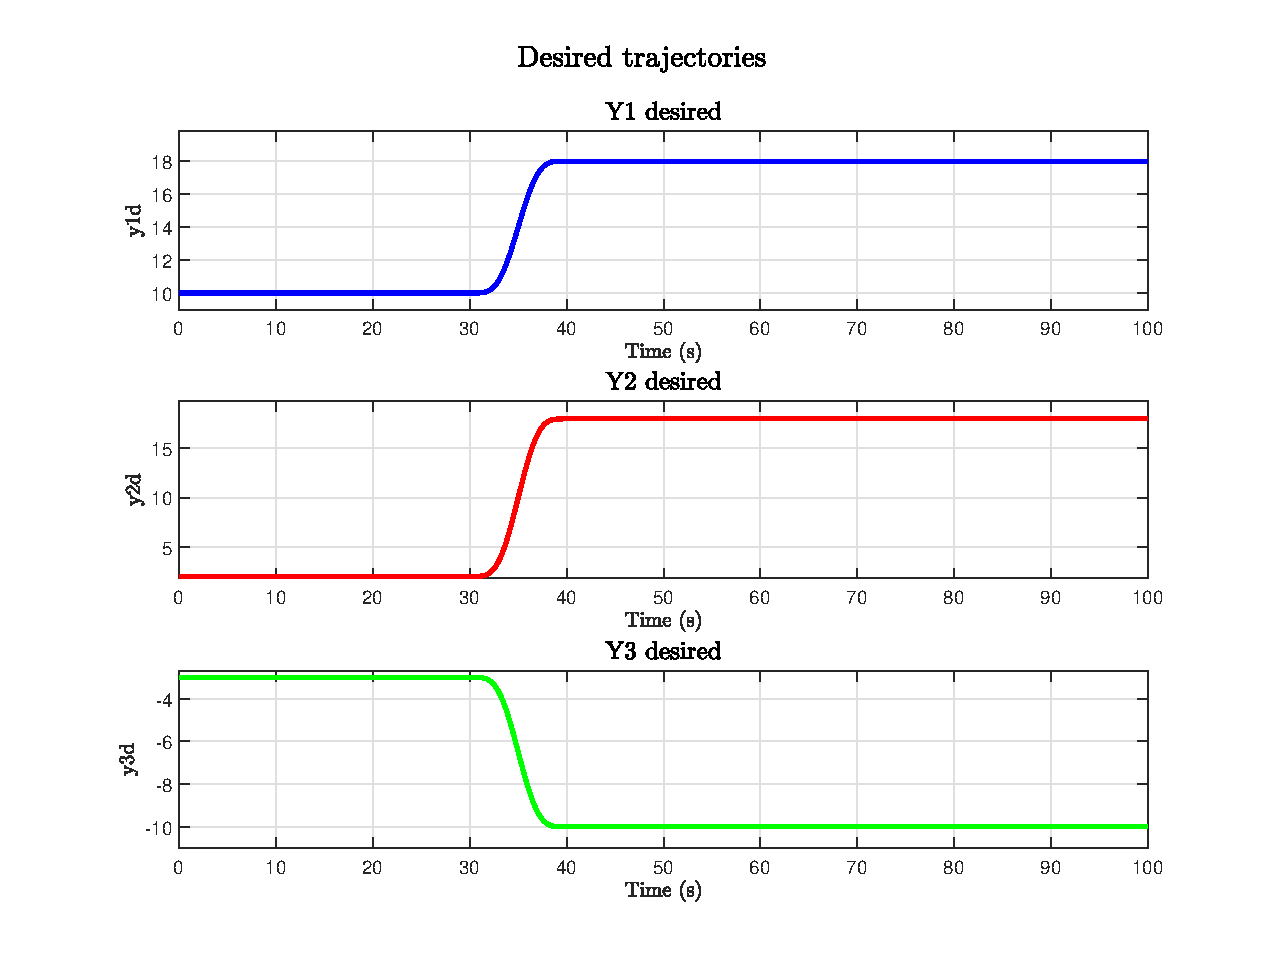
\includegraphics[width=0.75\linewidth]{imgs/section1/desiredTraj.eps}
    \caption{Desired trajectories of the load.}
    \label{fig:Desired_Trajectory}
\end{figure}

The Figure~\ref{fig:XY_Trajectory} shows the desired and actual (only for MFC) trajectories of the load in 
the \(xy\)-plane to get a better view of the trajectory tracking and the difference at the initial time.

\begin{figure}[htbp]
    \centering
    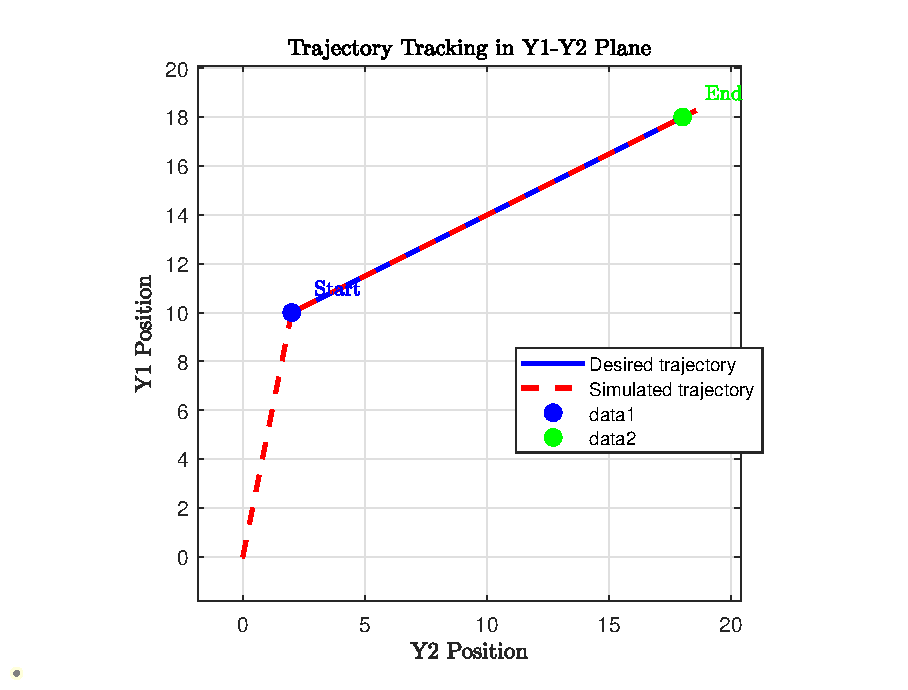
\includegraphics[width=0.8\linewidth]{imgs/section1/XYTrajectory.eps}
    \caption{Difference between desired states and model states.}
    \label{fig:XY_Trajectory}
\end{figure}

The next two figures Fig~\ref{fig:Input_High_Gain} and Fig~\ref{fig:Input_MFC} show the control inputs for 
both strategies.

\begin{figure}[htbp]
    \centering
    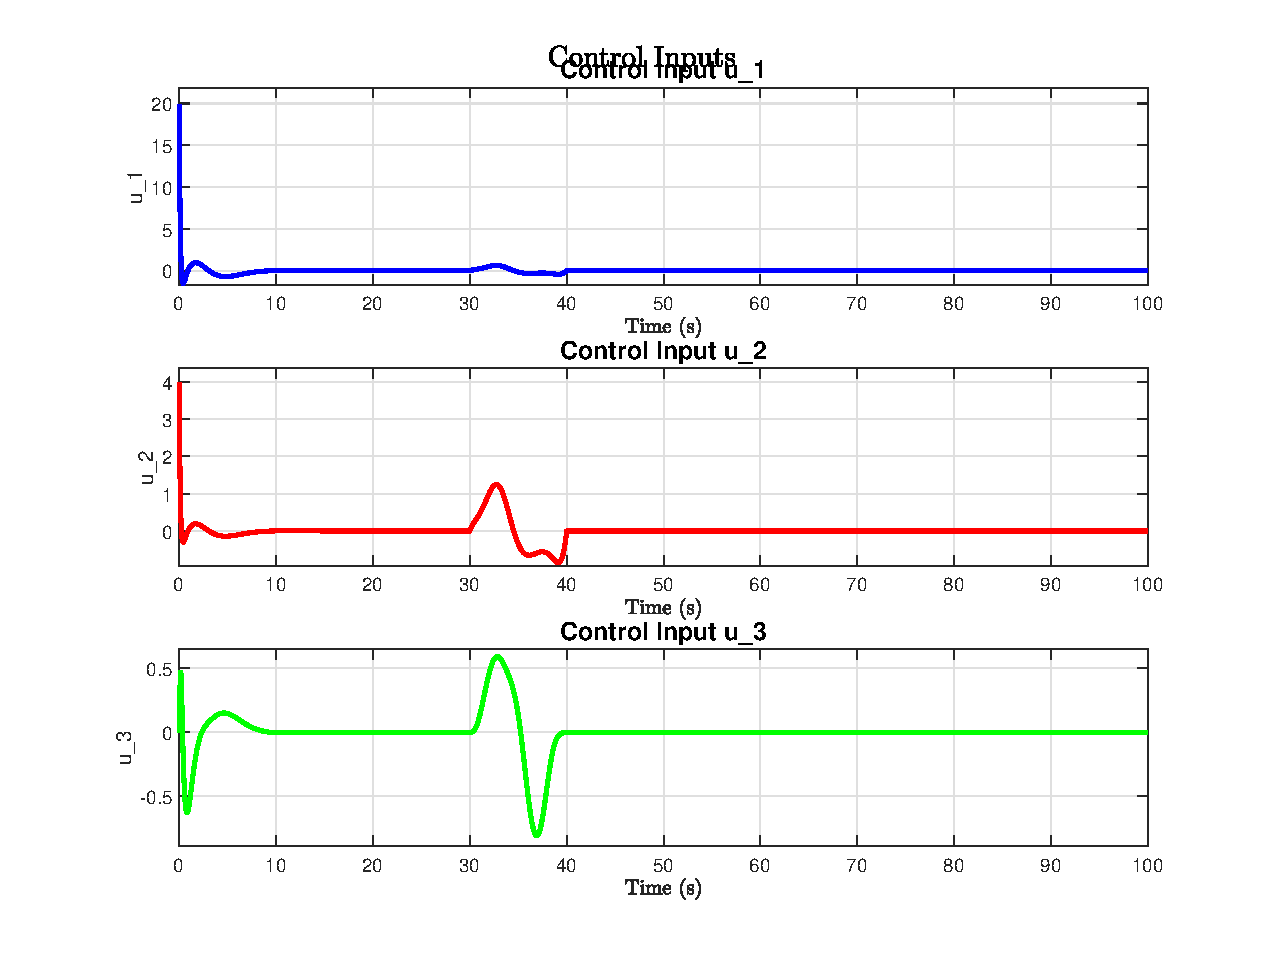
\includegraphics[width=0.8\linewidth]{imgs/section1/u_HG.eps}
    \caption{Input for set-point tracking using high-gain control.}
    \label{fig:Input_High_Gain}
\end{figure}

\begin{figure}[htbp]
    \centering
    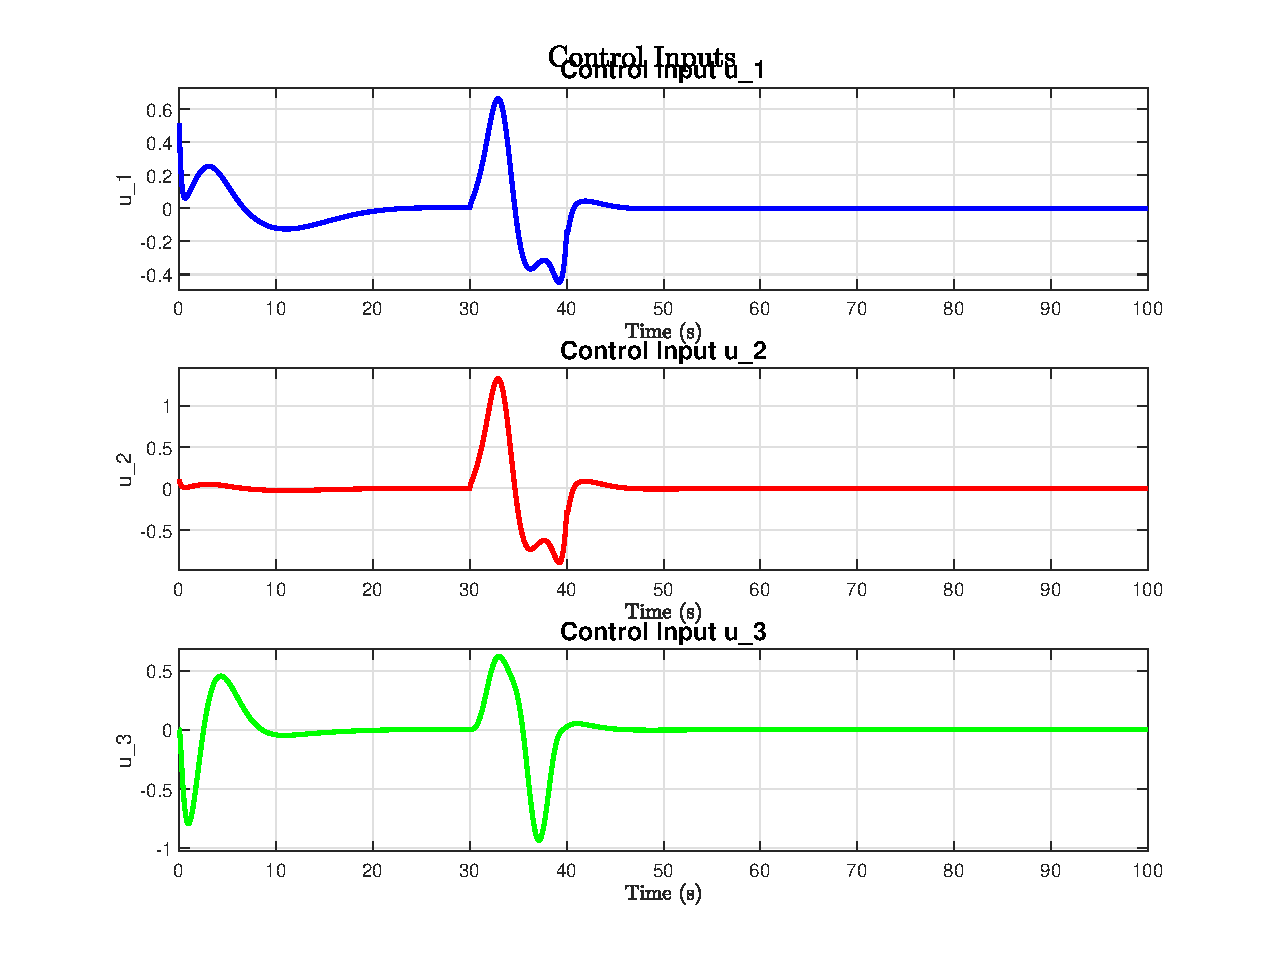
\includegraphics[width=0.8\linewidth]{imgs/section1/u_efficientMFC_Good_CI.eps}
    \caption{Input for set-point tracking using MFC.}
    \label{fig:Input_MFC}
\end{figure}

One can see that behaviors of both controllers aligns well with the predictions with a peak at \(t = 0\) for 
the High Gain control strategy and a reasonable input for the MFC strategy.

Now we can focus on the real plant experiment to see if the theory holds in a real environment with the environment
D-Space control Desk.

\newpage
\subsection{Real Plant Experiment}

We can see on figures~\ref{fig:Trolley_Zoom}, \ref{fig:X_Motor_Zoom} 
and \ref{fig:Y_Motor_Zoom} the the real plant crane system used for the
experimentation.

All of the control have been implemented on a 2011 version of Matlab Simulink
then compiled on D-space control desk. I won't go into the details of the
implementation on D-space because it is not the goal of this report but here 
in appendix \ref{app:Dspace_implementation} is an overview of the steps needed
to launch the control on the real plant.

\begin{figure}[htbp]
    \centering
    \rotatebox{270}{\includegraphics[width=0.5\linewidth]{imgs/section1/Trolley.jpg}}
    \caption{Zoom on the crane's trolley.}
    \label{fig:Trolley_Zoom}
\end{figure}

\begin{figure}[htbp]
    \begin{subfigure}{0.5\textwidth}
        \centering
        \rotatebox{270}{\includegraphics[width=\linewidth]{imgs/section1/Xmot.jpg}}
        \caption{Zoom on X motor.}
        \label{fig:X_Motor_Zoom}
    \end{subfigure}
    \hfill
    \begin{subfigure}{0.5\textwidth}
        \centering
        \rotatebox{270}{\includegraphics[width=\linewidth]{imgs/section1/Ymot.jpg}}
        \caption{Zoom on Y motor.}
        \label{fig:Y_Motor_Zoom}
    \end{subfigure}
    \caption{Zoom on the crane's X and Y motors.}
    \label{fig:Motors_Zoom}
\end{figure}


With this crane system, we implemented the same kind of trajectory to 
test the peaking phenomenon. The values aren't the same but method remains.
The figures ~\ref{fig:Real_PLant_without_Peaking} and 
~\ref{fig:Real_Plant_with_Peaking} highlight the peaking phenomenon
presence in the MFC control when the initial condition of the model aren't
taken close enough to the desired trajectory, the control behaves like a
High Gain and the high input work is present at the beginning as we can 
see on figure ~\ref{fig:Real_Plant_with_Peaking}.


\begin{figure}[htbp]
  \centering
  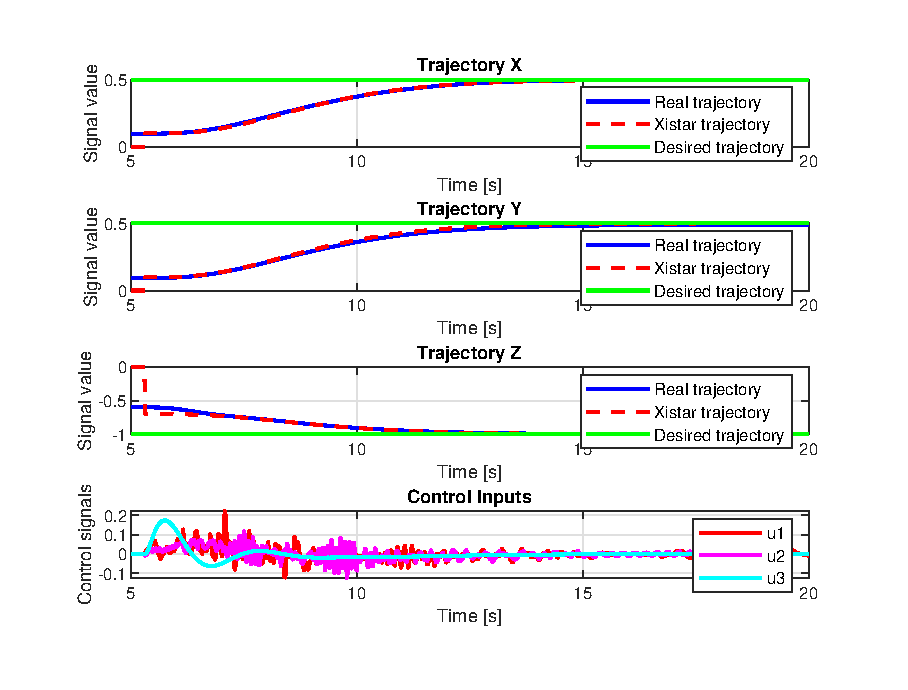
\includegraphics[width=0.8\linewidth]{imgs/section1/noPeaking.eps}
  \caption{Real plant experiment - trajectory tracking without peaking phenomenon.}
  \label{fig:Real_PLant_without_Peaking}
\end{figure}


\begin{figure}[htbp]
  \centering
  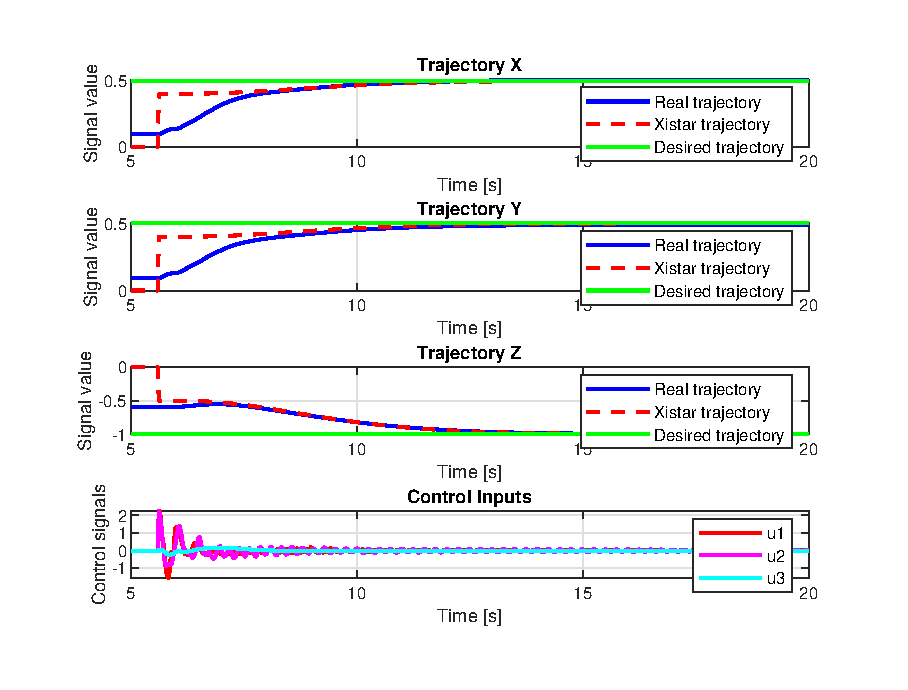
\includegraphics[width=0.8\linewidth]{imgs/section1/midPeaking.eps}
  \caption{Real plant experiment - trajectory tracking with peaking phenomenon.}
  \label{fig:Real_Plant_with_Peaking}
\end{figure}


The set points are reached in both cases with and exponential convergence that 
can be tuned with the time scaling factor \(\epsilon\).


\newpage
\section{Conclusion on the MFC Strategy}
The Model Following Control (MFC) strategy has been presented as a 
robust control technique that ensures a system's output follows a desired 
reference model, even in the presence of uncertainties and disturbances. 
This chapter detailed the theoretical foundations and implementation 
aspects of MFC, emphasizing its two-loop structure: the Model Control 
Loop (MCL) and the Process Control Loop (PCL). The MCL provides nominal 
control based on a theoretical model of the plant, while the PCL compensates 
for perturbations and model uncertainties.

The application of MFC to a crane system demonstrated its effectiveness in 
mitigating the peaking phenomenon, a common issue in high gain control 
strategies. The crane system was modeled with its full nonlinear dynamics, 
and feedback linearization was applied to achieve precise control. The 
simulation results and real plant experiments highlighted the advantages 
of MFC over High Gain control. Specifically, MFC reduced the peaking 
phenomenon and required less input work, making it more suitable for 
real-world applications.

The simpler design of MFC, as proposed by Tietze et al., was also discussed 
and implemented. This design streamlined the control loop dynamics, making 
the control law easier to implement and understand. The simulation and 
experimental results confirmed that the simpler design maintained the 
performance benefits of the original MFC strategy while reducing complexity.

In conclusion, the MFC strategy offers a robust and effective solution 
for systems where precise tracking of a reference trajectory is essential. 
It mitigates the peaking phenomenon, reduces input work, and provides a 
simpler control law compared to traditional high gain control strategies. 
Future work could explore further simplifications of the control architecture 
and the application of MFC to other complex systems.

\newpage



\chapter{Local Stability of high order super-twisting with time and state dependent perturbations}

\section{Introduction} 

This chapter presents the other problem I had to work on during my internship. It is based on the articles by my supervisor \cite{tietze2024local}, \cite{tietze2024localStabilisation}, and \cite{tietze2025dynamic}. The work starts from the reflection that in the proof given in the previous work on the sliding mode algorithm \cite{Moreno2012}, the perturbation is assumed to be bounded and only time dependent. This is a strong assumption, as in many practical cases, the perturbation can depend on the state of the system which leads to the creation of an algebraic loop. Let's consider the r-th order perturbed chain of integrators:

\begin{equation}
    \label{eq:perturbed_chain}
    (S) \qquad \dot{z} = J_r z + (\Delta(t,z) + u) e_r, \quad z = (z_1, z_2, \ldots, z_r) \in \mathbb{R}^r, \; u \in \mathbb{R}
\end{equation}

where $J_r$ is the r-th Jordan block, $e_r = (0, \ldots, 0, 1)^T \in \mathbb{R}^r$ and 
$\Delta: \mathbb{R}_+ \times \mathbb{R}^r \to \mathbb{R}$ is a perturbation. The goal is to design a 
feedback law $u = u(t,z)$ such that the closed-loop system is finite time stable with respect to the origin.

The work initiated by \cite{tietze2024local}, \cite{tietze2024localStabilisation} and 
\cite{tietze2025dynamic} took different variations of the Sliding Mode control (SMC) algorithm and sucessfully
proved the local finite time stability of the closed loop system. Here we are looking for the 
same kind of proof on the same model but for the High Order Super Twisting algorithm (HOST).

Several work already exist on he stability of HOST with time and state dependent perturbation, like 
\cite{Moreno2012} for the classical Super Twisting algorithm or \cite{kamal2014higher} which extend the
case the the r-th order. However, the proof is not complete as it does not take into account the
algebraic loop created by the state dependence of the perturbation.

The results presented in \cite{Laghrouche2017} on a different kind of HOST algorithm, gives a proof
of global finite time convergence with the HOST defined in \cite{Hong2005}. However the proof is
not done on a time and state dependent perturbation and uses a different strategy than the one used in
\cite{khalil2002nonlinear} based on invariant sets constrained by a Lyapunov function.


\newpage
\section{Context and problem statement}

We consider the perturbed chain of integrators defined in \eqref{eq:perturbed_chain} with a perturbation
$\Delta(t,z)$ satisfying the following assumption:

\begin{equation}
    \label{eq:assumption_perturbation_sum}
    \Delta(t,z) = \Delta_t(t) + \Delta_z(z)
\end{equation}

where $\Delta_t: \mathbb{R}_+ \to \mathbb{R}$ is a time dependent perturbation and 
$\Delta_z: \mathbb{R}^r \to \mathbb{R}$ is a state dependent perturbation. We assume that the state \(z(t)\) 
is always available for control. The initial value of the system is denoted by \(z_0 = z(0) \in \mathbb{R}^r\). 

The Goal is to design a feedback law \(u = u_{st}(t,z)\) such that the closed-loop system is finite time stable
with respect to the origin \(z = 0\).

First, we will analyse the control law given in \cite{Laghrouche2017} and \cite{Hong2005} and their stability
proof. Then we will try to adapt this vision to our problem and see if we can get to this result by 
taking into account the state dependent perturbation.

\subsection{High Order Super Twisting algorithm}

First of all, let's define the HOST algorithm as in \cite{Laghrouche2017}.

The following uses a results on stabilization theory on \ref{eq:perturbed_chain} as well as a geometric condition on the
homogeneous stabilizing feedback.

Let \(\mathcal{K} < 0\) and \(p > 0\) with \( p + (r + 1)\kappa \geq 0 \), set 
\( \pi_i := p + (i - 1)\kappa \), \( 1 \leq i \leq r + 1 \). For \( \epsilon > 0 \), let 
\( \delta_{\epsilon} : \mathbb{R}^r \rightarrow \mathbb{R}^r \) and \( \psi_{\epsilon} :
 \mathbb{R}^{r+1} \rightarrow \mathbb{R}^{r+1} \) be the family of dilations associated 
 with \( (p_1, \ldots, p_r) \) and \( (p_1, \ldots, p_{r+1}) \) respectively.


\begin{Proposition}
\label{prop:stabilizing_feedback}
Let \( r \) be a positive integer. There exists a feedback law \( u_0 : \mathbb{R}^r \to \mathbb{R} \), 
homogeneous of degree \( p_r + 1 \) with respect to \( (\delta_\epsilon)_{\epsilon > 0} \) such that the 
closed-loop system (CI)\textsuperscript{r} with \( u_0 \) is finite time stable and the following conditions 
hold true:

\begin{enumerate}
    \item The function \( z \mapsto Jr z + u_0(z) e_r \) is homogeneous of degree \( \kappa \) with 
    respect to \( (\delta_\epsilon)_{\epsilon > 0} \), and there exists a continuous positive definite 
    function \( V_1: \mathbb{R}^r \to \mathbb{R}_+ \), \( C^1 \) except at the origin, homogeneous with 
    respect to \( (\delta_\epsilon)_{\epsilon > 0} \) of degree \( 2p_r + 1 \) such that there exists 
    \( c > 0 \) and \( \alpha \in (0, 1) \) for which the time derivative of \( V_1 \) along non-trivial 
    trajectories of (CI)\textsuperscript{r} verifies \( \dot{V}_1 \leq -cV_1^\alpha \).
    \item \( z \mapsto \partial_r V_1(z) \) is homogeneous of positive degree with respect 
    to \( (\delta_\epsilon)_{\epsilon > 0} \) and \( z \mapsto \partial_r V_1(z)u_0(z) \) is 
    negative over \( \mathbb{R}^r \).
\end{enumerate}


\end{Proposition}


We will take \( \alpha \) equal to : \( 1 + \frac{\kappa}{2p_r + 1} = \frac{1}{2} \) to get homogeneity properties
for a Lyapunov function to be used in the proof and a condition that assure finite time convergence.

\( \partial_r V_1 \) is homogeneous with respect to \( (\delta_\epsilon)_{\epsilon > 0} \) of 
degree \( p + (r + 1)\kappa = 0 \). In \cite{Hong2005}, a feedback law \( u_0: \mathbb{R}^r \to \mathbb{R} \) 
satisfying Condition (1) of Prop.\ref{prop:stabilizing_feedback} is explicitly built.

Now we can define the HOST algorithm as follows:

\begin{theorem}
    Consider the homogeneous mapping $u_0 : \mathbb{R}^r \rightarrow \mathbb{R}$ and the continuous positive 
    definite function $V_1 : \mathbb{R}^r \rightarrow \mathbb{R}_+$ provided by Proposition 1. For every 
    $k_P \geq 1$ and $k_I > 0$, let $u_{ST}(\cdot)$ be the dynamic state-feedback controller defined by

    \begin{align}
        u_{ST}(t) &= k_P u_0(z(t)) + k_I \xi(t) \label{eq:u_ST} \\
        \dot{\xi}(t) &= -k_I \partial_r V_1(z(t)), \quad \xi(0) = 0 \label{eq:xi_dot} 
    \end{align}

    and we refer to $u_{ST}$ as the \textit{HOST} controller. The feedback connection between 
    \ref{eq:perturbed_chain} with the assumption \(\Delta(t, z) = 0\) and \eqref{eq:u_ST} gives rise to the 
    dynamical system over $\mathbb{R}^{r+1}$ given by

    \begin{align}
        \dot{z}(t) &= J_r z(t) + (k_P u_0(z(t)) + k_I \xi(t)) e_r \label{eq:z_dot} \\
        \dot{\xi}(t) &= -k_I \partial_r V_1(z(t)), \quad \xi(0) = 0. \label{eq:xi_dot_system}
    \end{align}

    There exist $A, d > 0$ such that, if $W : \mathbb{R}^{r+1} \rightarrow \mathbb{R}$ is defined by

    \begin{equation}
        W(z, \xi) = \left(V_1(z) + \frac{\xi^2}{2}\right)^{2-\alpha} - A z_r \xi, \label{eq:W}
    \end{equation}

    then $W$ is positive definite, $C^1$ except at the origin, homogeneous with respect 
    to $(\psi_\varepsilon)_{\varepsilon > 0}$ and the time derivative of $W$ along non-trivial 
    trajectories of \eqref{eq:z_dot}-\eqref{eq:xi_dot_system} verifies $\dot{W} \leq -d W^{1/(2-\alpha)}$. 
    As a consequence, trajectories of \eqref{eq:z_dot}-\eqref{eq:xi_dot_system} converge to zero in finite 
    time, i.e., $u_{ST}$ stabilizes \ref{eq:perturbed_chain} in finite time.
\end{theorem}


This theorem gives a first framework for the stability proof of the HOST algorithm. Also we can notice that 
the control law and the condition on A and d are also given in \cite{Laghrouche2017}. The complete proof 
is not given in \cite{Laghrouche2017} but can be found in the appendix\ref{app:proof_theorem1} with 
the explicit values of A and d.

The next step in this work is to introduce the perturbation \(\Delta(t,z)\) in the closed loop system 
and see how it can be taken into account in the stability proof. With the assumption that the perturbation
only depends on time \(\Delta(t,z) = \Delta_t(t)\), and it is bounded with : 

\begin{equation}
    \label{eq:assumption_perturbation_time_forLagrouche}
    |\Delta_t(t)| \leq \delta, \quad |\dot{\Delta}_t(t)| \leq \delta_t, \quad \forall t \geq 0
\end{equation}

The solution given in \cite{Laghrouche2017} is to introduce a time scaling factor and by a change of
variable and by using the homogeneity properties of the system, we can prove the finite time stability of the
closed loop system. By considering the next theorem:

% \begin{theorem}
%     Consider the perturbed chain of integrators defined by \ref{eq:perturbed_chain}, where 
%     the perturbation \(\Delta\) assures the assumption \ref{eq:assumption_perturbation_time_forLagrouche}. 
%     Assume that there exists a continuous homogeneous feedback law \(u_0\) and a Lyapunov function \(V_1\) 
%     verifying the assumptions (1) and (2) of Proposition \ref{prop:stabilizing_feedback} with \(p+(r+1)\kappa=0\). 
%     Then, for every positive gains \(k_P \geq 1\) and \(k_I > 0\), there exists \(\lambda_0 > 0\) only 
%     depending on the gains and \(\delta_t\) such that, for \(\lambda \geq \lambda_0\), the dynamic 
%     state-feedback controller \(u_{ST}^{\lambda}(\cdot)\) defined by

%     \begin{align}
%         \label{eq:u_ST_lambda}
%         u_{ST}^{\lambda}(t) &= \left(k_P u_0(D_{\lambda} z(t)) + k_I \xi^{\lambda}(t)\right) \\
%         \dot{\xi}^{\lambda}(t) &= -\lambda k_I \partial_r V_1(D_{\lambda} z(t)), \quad \xi^{\lambda}(0) = 0
%     \end{align}
    
%     where \(D_{\lambda} = \text{diag}(\lambda^{r-1}, \ldots, \lambda, 1)\) and stabilizes \ref{eq:perturbed_chain} in finite-time. In particular, \(u_{ST}^{\lambda}(\cdot)\) is continuous.
% \end{theorem}

% Fix \(k_P \geq 1\) and \(k_I > 0\). For every \(\lambda > 0\), consider the standard time-coordinate 
% change of variable along trajectories of \ref{eq:perturbed_chain} defined by \(y(t) = D_{\lambda} z(t/\lambda)\). 
% Under the hypotheses of the theorem, \ref{eq:perturbed_chain} can be rewritten as 

% \begin{equation}
%     \label{eq:perturbed_chain_scaled}
%     \dot{y} = J_r y + (u_{\lambda} + \Delta_{\lambda}) e_r
% \end{equation}

% where one has set, for \(t \geq 0\), \(u_{\lambda}(t) := u(t/\lambda)\) and \(\Delta_{\lambda}(t) := \Delta(t/\lambda)\) with \(|\dot{\Delta}_{\lambda}| \leq \Delta_t/\lambda\).

% The feedback connection between \ref{eq:perturbed_chain} and \ref{eq:u_ST_lambda} can be written as the 
% time-varying system over \(\mathbb{R}^{r+1}\) given by

% \begin{align}
%     \label{eq:closed_loop_perturbed_scaled}
%     \dot{y}(t) &= J_r z(t) + \left(k_P u_0(y(t)) + k_I \xi_{\lambda}(t)\right) e_r \\
%     \dot{\xi}_{\lambda}(t) &= -k_I \partial_r V_1(y(t)) + \dot{\Delta}_{\lambda}, \quad \xi_{\lambda}(0) = \Delta_{\lambda}(0)
% \end{align}

% where \(\xi_{\lambda}(t) = \xi^{\lambda}(t/\lambda) + \Delta_{\lambda}(t)\).

% Clearly, \ref{eq:closed_loop_perturbed_scaled} corresponds to the differential 
% inclusion \ref{eq:z_dot}-\ref{eq:xi_dot_system} perturbed by the time-varying vector field over 
% \(\mathbb{R}^{r+1}\) given by \((0, \cdots, 0, \dot{\Delta}_{\lambda}(t))^T\) or, equivalently, by 
% the multifunction : 

% \begin{equation}
%      (0, \cdots, 0, [-\Delta_t/\lambda, \Delta_t/\lambda])^T
% \end{equation}

% ,taking values in the subsets of \(\mathbb{R}^{r+1}\). Let \(W\) be the Lyapunov function defined in \ref{eq:W}. 
% Along non trivial trajectories of \ref{eq:closed_loop_perturbed_scaled}, one gets, for every \(t \geq 0\), that : 

% \begin{equation}
%     \dot{W} \leq -dW^{2/3} + \partial_{\xi}W \dot{\Delta}_{\lambda}(t) \leq -dW^{2/3} + \Delta_t|\partial_{\xi}W|/\lambda
% \end{equation}

% According to Remark 1, the homogeneity degree of \(|\partial_{\xi}W|\) is equal to 
% \(3p_{r+1} - p_{r+1} = 2p_{r+1}\), i.e., the homogeneity degree of \(W^{2/3}\). One deduces from the 
% previous equation that there exists \(\Delta_* > 0\) such that \(\dot{W} \leq -dW^{2/3}/2\), along 
% trajectories of System \ref{eq:closed_loop_perturbed_scaled} if \(\Delta_t/\lambda \leq \Delta_*\), i.e., 
% \(\lambda \geq \lambda_0 = \Delta_t/\Delta_*\). Hence the conclusion.


% The contents of Theorem 2 can be derived without relying on HOST controllers but rather on extending the 
% relative degree of the original system. The latter techniques, however, require a longer chain of integrators. 
% Notice that the choice of \(\lambda_0\) can be made explicit once \(u_0\) and \(V_1\) are explicitly given. 
% We do not know how to extend the above result to cases where \(p+(r+1)\kappa>0\). Indeed, for the above 
% homogeneity argument to work, it is necessary that \(W^{1/(2-\alpha)}\) (with \(\alpha=1/2\)) has the same 
% degree of homogeneity as \(\partial_{\xi}W\) since \(\dot{\Delta}\) is simply bounded. On the other hand, 
% \(W^{1/(2-\alpha)}\) has the same degree of homogeneity as \(\partial_{\xi}W \xi\) and thus \(\partial_r V_1\) 
% must necessarily be of degree zero. This occurs only if \(p+(r+1)\kappa=0\).

% \subsection{Modified Theorem}

Consider the perturbed chain of integrators defined by Equation \ref{eq:perturbed_chain}, where the 
perturbation \(\Delta\) satisfies assumption \ref{eq:assumption_perturbation_time_forLagrouche}.

Assume there exists a continuous homogeneous feedback law \(u_0\) and a Lyapunov 
function \(V_1\) satisfying the following assumptions (1) and (2) of Proposition 
\ref{prop:stabilizing_feedback} with \(p+(r+1)\kappa=0\):

\begin{enumerate}
    \item The function \( z \mapsto Jr z + u_0(z) e_r \) is homogeneous with respect 
    to \((\delta_\epsilon)_{\epsilon > 0}\), and there exists a continuous positive definite 
    function \( V_1: \mathbb{R}^r \to \mathbb{R}_+ \), \( C^1 \) except at the origin, homogeneous 
    with respect to \((\delta_\epsilon)_{\epsilon > 0}\).

    \item \( z \mapsto \partial_r V_1(z) \) is homogeneous of positive degree with respect 
    to \((\delta_\epsilon)_{\epsilon > 0}\) and : \begin{equation} z \mapsto \partial_r V_1(z)u_0(z) \end{equation} is negative 
    over \(\mathbb{R}^r\).
\end{enumerate}

We have the following theorem:

\begin{theorem}
    For every positive gains \(k_P \geq 1\) and \(k_I > 0\), there exists \(\lambda_0 > 0\) depending only 
    on the gains and \(\delta_t\) such that, for \(\lambda \geq \lambda_0\), the dynamic state-feedback 
    controller \(u_{ST}^{\lambda}(\cdot)\) defined by

    \begin{align}
        u_{ST}^{\lambda}(t) &= \left(k_P u_0(D_{\lambda} z(t)) + k_I \xi^{\lambda}(t)\right) \label{eq:u_ST_lambda} \\
        \dot{\xi}^{\lambda}(t) &= -\lambda k_I \partial_r V_1(D_{\lambda} z(t)), \quad \xi^{\lambda}(0) = 0
    \end{align}

    where \(D_{\lambda} = \text{diag}(\lambda^{r-1}, \ldots, \lambda, 1)\), stabilizes \ref{eq:perturbed_chain} 
    in finite-time. In particular, \(u_{ST}^{\lambda}(\cdot)\) is continuous.
\end{theorem}

Fix \(k_P \geq 1\) and \(k_I > 0\). For every \(\lambda > 0\), consider the standard time-coordinate change 
of variable along trajectories of \ref{eq:perturbed_chain} defined by \(y(t) = D_{\lambda} z(t/\lambda)\). 
Under the theorem's hypotheses, \ref{eq:perturbed_chain} can be rewritten as:

\begin{equation}
    \dot{y} = J_r y + (u_{\lambda} + \Delta_{\lambda}) e_r
\end{equation}

where for \(t \geq 0\), \(u_{\lambda}(t) := u(t/\lambda)\) and \(\Delta_{\lambda}(t) := \Delta(t/\lambda)\) with \(|\dot{\Delta}_{\lambda}| \leq \Delta_t/\lambda\).

The feedback connection between \ref{eq:perturbed_chain} and \ref{eq:u_ST_lambda} can be written as the 
time-varying system over \(\mathbb{R}^{r+1}\) given by:

\begin{align}
    \dot{y}(t) &= J_r z(t) + \left(k_P u_0(y(t)) + k_I \xi_{\lambda}(t)\right) e_r \\
    \dot{\xi}_{\lambda}(t) &= -k_I \partial_r V_1(y(t)) + \dot{\Delta}_{\lambda}, \quad \xi_{\lambda}(0) = \Delta_{\lambda}(0)
    \label{eq:closed_loop_perturbed_scaled}
\end{align}

where \(\xi_{\lambda}(t) = \xi^{\lambda}(t/\lambda) + \Delta_{\lambda}(t)\).

Clearly, \ref{eq:closed_loop_perturbed_scaled} corresponds to the differential 
inclusion \ref{eq:z_dot}-\ref{eq:xi_dot_system} perturbed by the time-varying vector field 
over \(\mathbb{R}^{r+1}\) given by \((0, \cdots, 0, \dot{\Delta}_{\lambda}(t))^T\) or, equivalently, 
by the multifunction:

\begin{equation}
     (0, \cdots, 0, [-\Delta_t/\lambda, \Delta_t/\lambda])^T
\end{equation}

Let \(W\) be the Lyapunov function defined in \ref{eq:W}. Along non-trivial trajectories 
of \ref{eq:closed_loop_perturbed_scaled}, one gets, for every \(t \geq 0\), that:

\begin{equation}
    \dot{W} \leq -dW^{2/3} + \partial_{\xi}W \dot{\Delta}_{\lambda}(t) \leq -dW^{2/3} + \Delta_t|\partial_{\xi}W|/\lambda
\end{equation}

According to Remark 1 of \cite{Laghrouche2017}, the homogeneity degree of \(|\partial_{\xi}W|\) is equal 
to \(3p_{r+1} - p_{r+1} = 2p_{r+1}\), i.e., the homogeneity degree of \(W^{2/3}\). One deduces from 
the previous equation that there exists \(\Delta_* > 0\) such that \(\dot{W} \leq -dW^{2/3}/2\), along 
trajectories of System \ref{eq:closed_loop_perturbed_scaled} if \(\Delta_t/\lambda \leq \Delta_*\), 
i.e., \(\lambda \geq \lambda_0 = \Delta_t/\Delta_*\).

The contents of Theorem 2 can be derived without relying on HOST controllers, instead extending the 
relative degree of the original system. The latter approach, however, requires a longer chain of integrators.

Notice that the choice of \(\lambda_0\) can be made explicit once \(u_0\) and \(V_1\) are explicitly 
given. We do not know how to extend the above result to cases where \(p+(r+1)\kappa>0\). Indeed, for the 
above homogeneity argument to work, it is necessary that \(W^{1/(2-\alpha)}\) (with \(\alpha=1/2\)) has the 
same degree of homogeneity as \(\partial_{\xi}W\) since \(\dot{\Delta}\) is simply bounded. On the other 
hand, \(W^{1/(2-\alpha)}\) has the same degree of homogeneity as \(\partial_{\xi}W \xi\) and 
thus \(\partial_r V_1\) must necessarily be of degree zero. This occurs only if \(p+(r+1)\kappa=0\).

One remark we can make on the dilatation function and the necessary homogeneity of certain functions in the
assumptions is mandatory to get the conditions on A and d in the proof of Theorem 1 to extend the result
on the unit ball to a global stability with finite time convergence.

We now want to extend this result to the case where the perturbation is time and state dependent like in 
\ref{eq:assumption_perturbation_sum}. Unfortunately, the time scaling argument does not work in this case
because the term \(\lambda\) has no effect on the state dependent part of the perturbation derivative as 
we can see below:

\begin{equation}
    \dot{\Delta}(t) = \frac{\partial \Delta_t(t)}{\partial t} + \frac{\partial \Delta_t(t)}{\partial z} \dot{z}(t)
\end{equation}

so we got : 

\begin{equation}
    \dot{\Delta}_{\lambda}(t) = \frac{1}{\lambda} \frac{\partial \Delta_t(t)}{\partial t} + \frac{\partial \Delta_z(z(t))}{\partial z} \dot{z}
\end{equation}

It is easy to see that the second term is not affected by \(\lambda\) and thus we cannot use the same argument 
as before.

Now let's have a look on the work done in \cite{tietze2025dynamic} where the approach is different and deals 
with algebraic loops but only for a SMC Super Twisting algorithm.






















\subsection{The Super Twisting case with time and state dependent perturbation}

Now we will present the work done in \cite{tietze2025dynamic} on the Super Twisting algorithm with time and state
dependent perturbation. The goal is to estabilish a local stability result for the Super Twisting algorithm (STA)
and use the mathematical tools to try to get the same kind of result for the HOST algorithm.

The constrained sets with Lyapunov functions used in this work is also presented in \cite{khalil2002nonlinear}. 
Let's consider the following sections.


\subsubsection{Stability for Unbounded Perturbations : Sliding Mode case}

To construct an invariant measure for the functional \( V \), let
\(z = \begin{bmatrix} z_1 & z_2 \end{bmatrix}^T \in \mathbb{R}^n\) and \(\omega \in \mathbb{R}^n_\omega\).

We define the sliding variable:

\begin{align}
    s(z, \omega) &= Lz_1 + z_2 + H\omega \\
    \dot{\omega} &= Gz_1 + F\omega
\end{align}

With \( z_2 = s(z, \omega) - Lz_1 - H\omega \)

The dynamics are described by:

\begin{equation}
    \begin{cases}
        \dot{z}_1 = (A - BL)z_1 - BH\omega + Bs(z, \omega) \\
        \dot{s} = -\rho \text{sgn}(s(z, \omega)) + \Delta(z, t) \\
        \dot{\omega} = Gz_1 + F\omega
        \label{eq:closed_loop_dynamicNiclas}
    \end{cases}
\end{equation}

We consider the following Lyapunov function:

\begin{equation}
    V(z_1, \omega) = [z \quad \omega]^T P [z \quad \omega],
    \label{eq:Lyapunov_V}
\end{equation}

where \( P = P^T \geq 0 \) and \( A_{cl}^T P + P A_{cl} = -I \).
We also have:
\begin{equation}
    a = 2 \lambda_{\min}(P) \|P B\|_2.
\end{equation}
For a given \( c \geq 0 \), we define:

\begin{equation}
    \Omega_{c, c_\omega} = \left\{ \begin{pmatrix} z \\ \omega \end{pmatrix} \mid \|s(z, \omega)\| \leq c \text{ and } V(z, \omega) \leq c_\omega^2 \right\},
\end{equation}

where \( c_\omega > a c \).

We consider the following projection of the set \( \Omega_{c, c_\omega} \) on the z subset :

\begin{equation}
    \Psi_{c, c_\omega} = \left\{ z \mid \exists \omega \in \mathbb{R}^n_{\omega}, \begin{pmatrix} z \\ \omega \end{pmatrix} \in \Omega_{c, c_\omega} \right\}.
\end{equation}

Now, all the sets and condition are defined, we can state the main assumption and theorem of this section.

\begin{assumption}
    \label{assumption:H4}
    For given \( c \geq 0 \) and \( c_\omega \geq a c \), there exists \(\delta > 0\) such that 
    for all \(t \geq 0 \) and \( z \in \Psi_{c, c_\omega} \), then \( |\Delta(z, t)| \leq \delta \).
\end{assumption}


\begin{theorem}
    Consider the closed loop \ref{eq:closed_loop_dynamicNiclas} and assumption \ref{assumption:H4} 
    Given \( z(0) = z_0 \) and \( \omega(0) = \omega_0 \), with \( \rho > \delta \),
    Then:
    For all \((x_0, \omega_0) \in \Omega_{c, c_\omega}\), the solution \((z, \omega)\) is bounded and,
    \begin{equation}
        \begin{cases}
            &\forall t \geq 0, (z(t), \omega(t)) \in \Omega_{c, c_\omega} \\
            &\lim_{t \to \infty} (z(t), \omega(t)) \to 0 \\
            &s(z, \omega) = 0, \quad \forall t > t_0 = \min \{ t \geq 0 \mid s(z(t), \omega(t)) = 0 \}
        \end{cases}
    \end{equation}
\end{theorem}

This proof is very classical but gives a good framework for what is comming next with the introduction of the 
algebraic loop in the STA. The new assumption we are going to make only hold locally in the invariant sets 
and the theorem will be contructed on the same method.

The proof is given in the appendix \ref{app:ProofSMCLocalStabNiclas}.

\subsection{Stability for Unbounded Perturbations : Super Twisting case}

We have to consider the perturbation as the sum like in \ref{eq:assumption_perturbation_sum} 
: \( \Delta(z, t) = \Delta_z(z) + \Delta_t(t) \)

\textbf{Control Design} 

We use the classical STA with a gain scaling \(\mu > 0\) to compensate the perturbation:
\begin{equation}
    \begin{cases}
        u = u_0 - \mu^{-1} \alpha_1 |s(z, \omega)|^{1/2} \text{sgn}(s(z, \omega)) + v \\
        \dot{v} = -\frac{1}{2} \mu^{-2} \alpha_2 \text{sgn}(s(z, \omega)), \quad v(0) = v_0
    \end{cases}
\end{equation}

With the gains \( \alpha_1, \alpha_2 > 0 \), and the gain scale: \( \mu > 0 \).

This leads to the new closed loop dynamics:
\begin{equation}
    \begin{cases}
        \dot{z} = (A - BL)z_1 - BH\omega + B s(z, \omega) \\
        \dot{s} = -\mu^{-1} \alpha_1 |s(z, \omega)|^{1/2} \text{sgn}(s(z, \omega)) + v + \Delta(z, t) \\
        \dot{v} = -\frac{1}{2} \mu^{-2} \alpha_2 \text{sgn}(s(z, \omega)) \\
        \dot{\omega} = Gz_1 + F\omega
    \end{cases}
    \label{eq:closed_loop_dynamicNiclasSTA}
\end{equation}

\textbf{Stability of the Closed Loop} 

We have to create a new invariant set \(\Lambda_{c, c_\omega, \mu}\) for the extended state :
\((z, \omega, v) \in \mathbb{R}^{n + n_\omega + 1}\).

Given \( \alpha_1, \alpha_2 > 0 \), we note:

\begin{equation}
    A_s = \frac{1}{2} \begin{bmatrix} -\alpha_1 & 1 \\ -\alpha_2 & 0 \end{bmatrix}, \quad B_s = \begin{bmatrix} 0 \\ 1 \end{bmatrix}, \quad P_s = \begin{pmatrix} p_{11} & p_{12} \\ p_{12} & p_{22} \end{pmatrix}
\end{equation}

The solution of \( A_s^T P_s + P_s A_s = -I \) with \( p_{12} = -1 \).
Consider the following objective function:

\begin{equation}
V_\mu(s, v) = p_{11} |s| + 2 p_{12} \mu v |s|^{1/2} \text{sgn}(s) + p_{22} \mu^2 v^2
\end{equation}

We introduce also the compact set:

\begin{equation}
\Gamma_{c, \mu} = \left\{ \begin{pmatrix} s \\ v \end{pmatrix} \mid V_\mu(s, v) \leq k(c) \right\}
\end{equation}

where

\begin{equation}
k(c) = \frac{p_{11} p_{22} - p_{12}^2}{p_{22}} c
\end{equation}

We can show:
For \(\begin{pmatrix} s \\ v \end{pmatrix} \in \Gamma_{c, \mu}\), \(|s| \leq c\) and 
\(|v| \leq \frac{1}{\mu} \sqrt{\frac{p_{11}}{p_{22}}c}\).
Note: The upper bound of \(|v|\) increases when the value of \(\mu\) decreases and vice versa.
Therefore, for \(\forall \epsilon \in \mathbb{R}\):

\begin{equation}
    \exists v \in \mathbb{R}, \left( \begin{pmatrix} s \\ v \end{pmatrix} \in \Gamma_{c, \mu} \right) \iff |s| \leq c
\end{equation}

We consider the following Lyapunov function candidates \(V_\mu\) and \(V(z_1, \omega)\) \ref{eq:Lyapunov_V} 
and the scalar:
\begin{equation}
    a = 2 \lambda_{\max}^{1/2}(P) \|PB\|_2
\end{equation}

We define the following set:
\begin{equation}
    \Lambda{c, c_\omega, \mu} = \left\{ \begin{pmatrix} z \\ \omega \\ v \end{pmatrix} \mid V_\mu(s(z, \omega), v) \leq k(c) \cap V(z, \omega) \leq c_\omega^2 \right\}
\end{equation}

And their projections in the subspaces $z-\omega$ and $z$:

\begin{equation}
    \Phi_{c, c_\omega} = \left\{ \begin{pmatrix} z \\ \omega \end{pmatrix} \mid \exists v \in \mathbb{R}, \begin{pmatrix} z \\ \omega \\ v \end{pmatrix} \in \Lambda_{c, c_\omega, \rho} \right\}
\end{equation}
\begin{equation}
    \Psi_{c, c_\omega} = \left\{ z \mid \exists (\omega, v) \in \mathbb{R}^{m_\omega + 1}, \begin{pmatrix} z \\ \omega \\ v \end{pmatrix} \in \Lambda_{c, c_\omega, \rho} \right\}
\end{equation}

\begin{lemma}
The projections \(\Phi_{c, c_\omega}\) and \(\Psi_{c, c_\omega}\) don't depend on \(\mu > 0\) and 
\(\Phi_{c, c_\omega} = \Omega_{c, c_\omega}\) and
\(\Psi_{c, c_\omega} = \Psi_{c, c_\omega} \quad \forall c > 0 \text{ or } c_\omega > a c\).
\end{lemma}

Given a variable of comparison \(u_c\), \(\exists u_{\max} > 0\) independent of \(\mu\) such that:
\begin{equation}
    \|Az_1 + Bz_2\|_2 + |u_0| \leq u_{\max} \quad \forall \begin{pmatrix} z \\ \omega \end{pmatrix} \in \Phi_{c, c_\omega}
\end{equation}

\begin{assumption}
    For all \(c \geq 0\) and \(c_\omega \geq a c\), there exist \(\delta, \delta_t, \delta_z > 0\) such that 
    for all \(t \geq 0\) and all \(z \in \Phi_{c, c_\omega}\), we have:
    \begin{equation}
        |\Delta(z, t)| \leq \delta,
    \end{equation}
    \begin{equation}
        \left| \frac{d\Delta_t(t)}{dt} \right| \leq \delta_t,
    \end{equation}
    \begin{equation}
        \left| \frac{\partial \Delta_z(z)}{\partial z} \right| \leq \delta_{z} 
    \end{equation}
\end{assumption}

These lemma and assumption give the key to have conditions on the gain \(\mu\) to ensure the stability 
in case of unbounded perturbation. We can proove the next theorem by the same method as before with the 
invariant sets and the Lyapunov functions we created in this section. The proof can be found in \cite{tietze2025dynamic}.


\begin{theorem}
    Consider the Closed Loop of \ref{eq:closed_loop_dynamicNiclasSTA} and the Initial Conditions:

    \begin{equation} 
        z(0) = z_0, \quad \omega(0) = \omega_0, \quad v(0) = v_0 
    \end{equation}

    Let

    \begin{equation}
        \mu_0 = (\delta \|P_0 B_0\|_2)^{-1} \left( \frac{k(c)}{\lambda_{\min}(P_s)} \right)^{1/2},
    \end{equation}

    \begin{equation}
        \mu_1 = (2\gamma \|P_s B_s\|_2)^{-1}.
    \end{equation}

    For \(\gamma = \mu_0 (\delta_t + \delta_z U_{\max} + \delta_z \delta) + \delta_z (\alpha_1 + \sqrt{\frac{p_{11}}{p_{22}}})\sqrt{c}\),
    
    For all \(\mu < \min(\mu_0, \mu_1)\), and \(\begin{pmatrix} z_0 \\ \omega_0 \\ v_0 \end{pmatrix} \in \Lambda_{c, c_\omega, \rho}\), 
    the solution \((z, \omega, v)\) is bounded such that :

    \begin{equation}
        \forall t \geq 0, (z(t), \omega(t), v(t)) \in \Delta_{c, c_\omega, \rho},
    \end{equation}

    where \(\lim_{t \to \infty} (z(t), \omega(t)) = 0\), and \(\forall t \geq t_0 > 0\):
    
    \begin{equation}
        s(z(t), \omega(t)) = 0,
    \end{equation}
    
    \begin{equation}
        v(t) = -\Delta(z(t), t).
    \end{equation}
\end{theorem}


The use of the scaling gain \(\mu\) gives the possibility to compensate the perturbation and ensure the 
stability of the closed loop system with explicite conditions. The question is, can we use the same method 
to estabilish an invariant set on the HOST algorithm with the Lyapunov function given in \cite{Laghrouche2017} ?
Is it sufficient to also just add the scaling gain \(\mu\) in the HOST algorithm to ensure the stability in 
case of algebraic loop ?



%=========================================================================================================%
%                                                                                                         %
%                                      NEW SECTION                                                       %
%                                                                                                         %
%=========================================================================================================%
\newpage
\section{Algebraic Loops in High Order Super Twisting}

As we saw in the previous section, the Super Twisting algorithm case can be used in case of time and state dependent
perturbation with the introduction of an algebraic loop can be extend to the HOST algorithm. The work is divided
in two steps because of the complexity in the reunion of the two theorems using different tools and methods.

First, we will try to get a first result on a evident case with an easy to handle class of perturbation to 
get the theory right. Then we will try to extend the result to a more general class of perturbation

\subsection{First step : taking an easy class of perturbation to handle}

We consider the system of dimension \(r \in \mathbb{N}\) with the following dynamics:

\begin{equation}
    \dot{z} = J_r z + (u + \Delta(z, t)) e_r
\end{equation}

where \(z \in \mathbb{R}^r\), \(J_r\) is the \(r\)-order Jordan block, \(e_r = [0, \ldots, 0, 1]^T \in \mathbb{R}^r\),
\(u \in \mathbb{R}\) is the control input and \(\Delta(z, t)\) is a perturbation depending on the state and time.

The perturbation satisfies the following assumption:

\begin{assumption}
    \label{assumption:perturbation_easy_case}
    There exists \(\delta, \delta_z, \delta_t > 0 \) such that for all \( t \geq 0 \) and \( z \in \mathbb{R}^r \):
    \begin{equation}
        \Delta(z, t) = \Delta_z(z) + \Delta_t(t)
    \end{equation}
    and,
    \begin{equation}
        \forall z, t \in \mathbb{R}^r \times \mathbb{R}_+, \\
        \begin{cases}
            |\Delta(z, t)| \leq \delta, \\
            \left| \frac{d\Delta_t(t)}{dt} \right| \leq \delta_t, \\
            \forall i \in \{1, \ldots, r\}, \left| \frac{\partial \Delta_z(z)}{\partial z_i} \right| \leq \delta_{z}
        \end{cases}
    \end{equation}
\end{assumption}

We assume that there exists the same stabilizing feedback law \(u_0\) and Lyapunov function \(V_1\) as in
Proposition \ref{prop:stabilizing_feedback} with \(p + (r+1)\kappa = 0\) and \(\alpha = 1 + \frac{\kappa}{2p_{r+1}} =1/2\).


The next assumption is the one that differentiate this section from the next one on the class of the perturbation.

\begin{assumption}
    \label{assumption:H4_extended}
    For all \(z \in \mathbb{R}^r\), we have : \(\frac{\partial \Delta_z(z)}{\partial z_r} = 0\)
\end{assumption}

This assumption is very strong and may be out of context because it is clear that it kills the algebraic loop :

\begin{equation}
    \dot{\Delta}(z, t) = \frac{d\Delta_t(t)}{dt} + \sum_{i=1}^{r} \frac{\partial \Delta_z(z)}{\partial z_i} \dot{z}_i = \frac{d\Delta_t(t)}{dt} + \sum_{i=1}^{r-1} \frac{\partial \Delta_z(z)}{\partial z_i} z_{i+1}
\end{equation}

Which doesn't contains the control input dynamics. We can state the following inequality independent 
of the control input:

\begin{equation}
    |\dot{\Delta}(z, t)| \leq \delta_t + \sum_{i=1}^{r-1} \delta_{z_i} |z_{i+1}| \leq \delta_t + \delta_z \|z\|_1
\end{equation}

And by placing us on the unit sphere and using the same notation as in the proof of 
Theorem in appendix~\ref{app:proof_theorem1} :

\begin{equation}
    |\dot{\Delta}(z, t)| \leq \delta_t + \sum_{i=1}^{r-1} \delta_{z_i} Z_{M_{i+1}} \leq \bar{\delta}
\end{equation}

with : \(Z_{M_i} = \max_{z \in R_p} |z_{i}|\)

But this case has an interest because even though \(\bar{\delta}\) doesn't depend on time and state,
the time scaling solution is no use here because of the state dependent part of the perturbation.

We consider the following HOST controller with a scaling gain \(\mu > 0\):
\begin{align}
    u_{ST}^{\mu}(t) &= \left(k_P u_0(z(t)) + k_I \xi^{\mu}_{\Delta}(t)\right) \\
    \dot{\xi}^{\mu}_{\Delta}(t) &= -\mu k_I \partial_r V_1(z(t)), \quad \xi^{\mu}_{\Delta}(0) = 0
\end{align}

Which leads to the closed loop dynamics:
\begin{equation}
    \begin{cases}
        \dot{z} &= J_r z + \left(k_P u_0(z) + k_I \xi^{\mu}_{\Delta}  \right) e_r \\
        \dot{\xi}^{\mu}_{\Delta} &= -\mu k_I \partial_r V_1(z(t)) + \dot{\Delta}(z, t), \quad \xi^{\mu}_{\Delta}(0) = \dot{\Delta}(0)
        \label{eq:closed_loop_dynamicNiclasHOST}
    \end{cases}
\end{equation}

The goal is to establish an invariant set constraining the system trajectories using the Lyapunov function 
\(W\) defined in \ref{eq:W}.

Let's consider the Lyapunov function \(W\) defined in \ref{eq:W} and the following set:
\begin{equation}
    \Lambda_{b, \mu} = \left\{ \begin{pmatrix} z \\ \xi \end{pmatrix} \mid W(z, \xi) \leq b \right\}
\end{equation}

We also cannot use the same approach as in \cite{Laghrouche2017} with the direct perturbed vector field.
The addition of the gain \(\mu\) has to be followed along the calculation to find a condition on it
that ensures the stability of the closed loop system.

The addition of the gain \(\mu\) in the HOST controller doesn't change the homogeneity of the closed loop system, so
we can stay on the unit sphere and compensate the perturbation with \(\mu\) like in the STA case by assuming this :

\begin{equation}
    \mu \leq 1 + \frac{\xi_{\max} \bar{\delta}}{(k_p - 1) V_{Umax}}
\end{equation}

where \(V_{Umax} = - \max_{z \in R_p} |\partial_r V_1(z) u_0(z)|\) and \(\xi_{\max} = \max_{\xi \in R_\xi} |\xi|\).

This assumption seems not very logical because it gives an upper bound on \(\mu\) but, we have to keep in mind
that \(\mu > 0\) to ensure the stability which creates a constraint on \(k_p\) that has to be sufficiently large to
ensure the existence of \(\mu\) and thus the stability of the closed loop system.

This assumption assures that the function \(W\) is a Lyapunov function for the closed loop system 
\ref{eq:closed_loop_dynamicNiclasHOST} and ensure that we can pursue the proof with the same method as in the 
last section with the STA using the invariant set \(\Lambda_{b, \mu}\) to establish the following theorem:

\begin{theorem}
    Consider the perturbed chain of integrators defined by the dynamics:
    \begin{equation}
    \dot{z} = J_r z + (u + \Delta(z, t)) e_r
    \end{equation}
    where the perturbation \(\Delta(z, t)\) satisfies Assumptions \ref{assumption:perturbation_easy_case} and \ref{assumption:H4_extended}. Assume there exists a continuous homogeneous feedback law \(u_0\) and a Lyapunov function \(V_1\) satisfying Proposition \ref{prop:stabilizing_feedback} with \(p + (r+1)\kappa = 0\) and \(\alpha = 1/2\).

    For every positive gains \(k_P \geq 1\) (that ensures the positiveness of \(\mu\)) 
    and \(k_I > 0\), and for a scaling gain \(\mu\) satisfying:

    \begin{equation}
        \mu \leq 1 + \frac{\xi_{\max} \bar{\delta}}{(k_p - 1) V_{Umax}}
    \end{equation}

    where \(V_{Umax} = - \max_{z \in R_p} |\partial_r V_1(z) u_0(z)|\) and \(\xi_{\max} = \max_{\xi \in R_\xi} |\xi|\), the dynamic state-feedback controller \(u_{ST}^{\mu}(\cdot)\) defined by:
    \begin{align}
        u_{ST}^{\mu}(t) &= \left(k_P u_0(z(t)) + k_I \xi^{\mu}_{\Delta}(t)\right) \\
        \dot{\xi}^{\mu}_{\Delta}(t) &= -\mu k_I \partial_r V_1(z(t)), \quad \xi^{\mu}_{\Delta}(0) = 0
    \end{align}
    ensures that the closed-loop system is finite-time stable with respect to the origin. 

\end{theorem}


\subsection{Second step : extending the result to a more general class of perturbation, main ideas}

I have not yet a complete result for this section but I will try to give the main ideas of the approach.

The main idea would be to consider the same system and controller as in the previous section but without
we can see quickly by following the same proof steps that the gain scaling \(\mu\) only in the integral part
of the HOST controller is not sufficient to compensate the perturbation derivative. A way should be to consider 
the new controller:

\begin{align}
    u_{ST}^{\mu}(t) &= \left(k_P u_0(z(t)) + \mu k_I \xi^{\mu}_{\Delta}(t)\right) \\
    \dot{\xi}^{\mu}_{\Delta}(t) &= -\mu k_I \partial_r V_1(z(t)), \quad \xi^{\mu}_{\Delta}(0) = 0
\end{align}

and try to mitigate the effects of the perturbation derivative with the gain \(\mu\) to keep the proprieties
of the Lyapunov function \(W\) defined in \ref{eq:W}. It would lead to the same conclusion.


Here the constion on the perturbation is different because we have to introduce the algebraic loop in its derivative:

\begin{align}
    \dot{\Delta}(z, t) &= \frac{d\Delta_t(t)}{dt} + \sum_{i=1}^{r} \frac{\partial \Delta_z(z)}{\partial z_i} \dot{z}_i \\
    &= \frac{d\Delta_t(t)}{dt} + \sum_{i=1}^{r-1} \frac{\partial \Delta_z(z)}{\partial z_i} z_{i+1} + \frac{\partial \Delta_z(z)}{\partial z_r} (k_P u_0(z) + \mu k_I \xi^{\mu}_{\Delta})
\end{align}

Here, we cannot find a bound \(\bar{\delta}\) independent of the state which complexifies a lot 
the calculations and the conditions on gain scaling \(\mu\) to ensure the stability of the closed loop system.

%=========================================================================================================%
%                                                                                                         %
%                                      NEW SECTION                                                       %
%                                                                                                         %
%=========================================================================================================%
\newpage
\section{Conclusion and future work}

Unfortunately, I didn't get enough time to finish the work on the HOST algorithm with algebraic loops
but I think the approach is correct and the first step is a good start to get the theory right. The next step
is to try to find gain scaling that fit the calculations to keep the Lyapunov function \(W\) as a Lyapunov 
function for the closed loop system. It is the easiest way to ensure the stability of the closed loop system that 
has the asset to stay close to the theory of \cite{tietze2025dynamic} with the ability to use the homogeneity
of the system to establish local invariant sets and extend the result to a global stability with finite time 
convergence.


The difficulty is to handle the unknown terms of the HOST controller that aren't very classical and 
create a condition on \( \mu \) that ensures the stability of the closed loop system while being 
possible because as we could have seen, the condition we can set on \( \mu \) in the first step have 
indirect repercussions on the choice of \( k_P \) and \( k_I \) that have to be sufficiently large to 
ensure the existence of \( \mu \) which increases the complexity of the tuning of the controller and the
work of the control input.

One last thing that I found very surprising is the lack of articles on the HOST algorithm especially on its
stability. The state of the art gives articles on its implementnation but few papers gives actual stability
proofs. The article \cite{Laghrouche2017} is the only one I found that gives a complete proof of the stability
of the HOST algorithm with a Lyapunov function that I could use and found very interesting to consider with
the work of \cite{tietze2025dynamic}.

%\input{Sections/section3}


\chapter{Personal Conclusion}

My internship at Technische Universität Ilmenau has been an enriching experience, both professionally and personally. Working within the Institut für Automatisierungs und Systemtechnik has provided me with valuable insights into advanced control systems and the practical challenges of implementing theoretical concepts in real-world scenarios.

On a professional level, I have gained significant experience in the field of sliding mode control and the resolution of algebraic loops. The collaborative environment and the expertise of my colleagues have greatly contributed to my understanding of complex control systems. I have also developed my research skills, including data analysis, simulation, and technical writing.

Culturally, living in Ilmenau has offered me a unique perspective on German life, particularly in the former East Germany. The blend of historical architecture and modern technological advancements at the university has been fascinating. The local culture, with its emphasis on efficiency and community, has left a lasting impression on me. Despite the occasional challenges with public transportation, such as the unreliable DeutschBahn, I have appreciated the simplicity and functionality of daily life in Ilmenau.

The academic environment at TU Ilmenau has been rigorous and focused on practical applications, which has enhanced my problem-solving skills and prepared me for future challenges in the field of control engineering. The interactions with my colleagues and the opportunity to work on cutting-edge research projects have been incredibly rewarding.

In conclusion, this internship has not only advanced my technical knowledge but also broadened my cultural horizons. It has reinforced my interest in pursuing a career in control systems and has provided me with valuable experiences that will benefit my future endeavors. I am grateful for the opportunity to have been a part of such a dynamic and innovative research team.
%======================= CONCLUSION =============================
\chapter*{Conclusion}
\addcontentsline{toc}{chapter}{Conclusion}

In the end, this internship has been on to very differnt topics. On one hand, the MFC I had to work on 
to implement it on a simulation and a real system. On the other hand, the algebraic loops which I would 
have like to go deeper but the time was not enough to do so.

The MFC is a very interesting control strategy, which has many assets compared to high gain control. And 
above all, its simplified definition is very quick to implement and quite independent of system parameters as 
it is used on linearized systems. In our case, we could extend the state to make the internal dynamics vanish but
as showed in \cite{Willkomm2023MFC}, if they are input-to-state stable, the MFC is totally applicable.
Its robustness and assets make it a very good candidate for industrial applications.

The algebraic loops resolution in sliding mode control approaches is a very interesting topic, which
introduced me to the scientific research in the filed of stability proofs and the real challenges 
of Lyapunov-based proofs. The method proposed in \cite{Laghrouche2017} is a good start for a certain class of
perturbations but the general case is still open. 

Finally, I regret not having been able to go deeper in this topic, as I would have liked to. And I want 
to acknowledge that it can be very important to state the conditions of the internship because some 
miscommunications led to a lack of supervising and I had to work mainly on my own which was sometimes challenging.
Especially when I had to work on the MFC topic which was not my main topic of the internship.


I'll also remember the cultural experience in Ilmenau, a small town in the former East Germany. The trip I could do 
during my free time in this country rich in history and culture. I could also learn again some German 
which was very nice and interesting.


\newpage

%récupérer les citation avec "/footnotemark"
\nocite{*}

%choix du style de la biblio
\bibliographystyle{plain}
%inclusion de la biblio
\bibliography{bibliographie.bib}
%voir wiki pour plus d'information sur la syntaxe des entrées d'une bibliographie

%Ne pas numéroter cette partie
\part*{Appendices}
%Rajouter la ligne "Appendices" dans le sommaire
\addcontentsline{toc}{part}{Appendices}
\appendix

\chapter{User notice to launch the MFC on the Real Plant of the Crane System}
\label{app:Dspace_implementation}
\section*{Initialization}
Here is a quick launch guide for the MFC control of the crane system.
\begin{enumerate}
    \item Open \textit{DSPACE ControlDesk 4.2.1}.
    
    \item Open the project and experiment located in the root directory:\\
    \textit{C:\textbackslash Users\textbackslash portalkran\textbackslash Documents\textbackslash MATLAB\textbackslash Crane User},\\
    and select \textit{Experiment\_001} of \textit{Project\_001}.
    
    \item Turn the real system ON (switch "Plant On") and wait for the \textbf{Ready to operate} indicator to light up in green. Then press \textbf{Servos On}.
    
    \item In ControlDesk, set the \textbf{StartNStop} value to 1 and press \textbf{Enable On} on the real system panel. The crane should then start moving to a corner at constant speed.
    
    \item Wait until the \textbf{initPhase} indicator reaches 1. Then, \textbf{controlAllowed} should also reach 1. This means that the system and controls are ready to operate.
    
    \item To start the MFC control, set \textbf{startCtrl} to 1. The crane will stabilize at the position : \((x_{pS},\ y_{pS},\ z_{pS})\)
\end{enumerate}
\section*{Dynamic Trajectories}
To start dynamic trajectory following, choose one by setting the value of \textit{enFF} to an integer between 1 and 4. The meaning of each value is:
\begin{itemize}
    \item \textbf{0}: No trajectory — the mass is stabilized at a fixed setpoint position.
    
    \item \textbf{1}: \textbf{1D sinusoidal motion along the \textit{x}-axis} — the mass oscillates smoothly back and forth along the horizontal axis (x-direction) following a cosine wave, while the y- and z-positions remain constant.
    \item \textbf{2}: \textbf{2D circular trajectory in the \textit{xy}-plane} — the mass follows a circular path centered near the setpoint in the horizontal plane (x-y). The vertical position remains fixed.
    \item \textbf{3}: \textbf{2D lemniscate (figure-eight) trajectory in the \textit{xy}-plane} — the mass follows a horizontally oriented lemniscate path (\(\infty\)-shaped) with smooth motion, centered around the setpoint. The vertical position remains fixed.
    \item \textbf{4}: \textbf{3D lemniscate trajectory with vertical oscillations} — the mass follows the same horizontal lemniscate (\(\infty\) shape) as in mode 3, but the z-axis position now varies sinusoidally. This creates a spatial 3D trajectory resembling a twisted ribbon or waving figure-eight path.
\end{itemize}
\section*{Last project with differentiator}
The last project made is from the file Matis Crane, which uses the MFC controller and the differentiator made by Niclas Tietze to estimate the states.
The Simulink model used to generate the code is in the file \textit{crane\_MFC\_Niclas\_DIFF.mdl}. To compile it, use the script \textit{build\_MFC\_crane\_Niclas.m}.
On DSPACE, open the project \textit{Project\_niclasDIFF} then experiment \textit{Experiment\_001}.
The parameters and board settings are quite similar to the previous version, except that we now use only one trajectory available in the block \textit{Niclas\_MFC/Desired Trajectory}.
One can set the first setpoint position of the trajectory by changing the values of the reference
\begin{itemize}
    \item \(x\_s = 0.2\)
    \item \(y\_s = 0.2\)
    \item \(l\_s = 0.4\)
\end{itemize}
{\sloppy In the block \textit{crane\_MFC\_Niclas\_DIFF/Portal Crane System/Crtl Selector/LQR/control algorithm}}

{\sloppy The control gains and parameters can be adjusted in the compiling script: \\
\textit{build\_MFC\_crane\_Niclas.m}.}

Finally, the control on DSPACE works basically the same as before:
\begin{itemize}
    \item Initialize the system by setting on one the control init button.
    \item The crane should go by itself in the left upper corner, if the Z-axis doesn't go up, look on the direct control app of the computer to put the signal type of the Z-axis to 0.
    \item Wait until the init phase is done and the control allowed is on, after that the LQR control block should stabilize the crane at the set point position (the block is available in: \textit{crane\_MFC\_Niclas\_DIFF/Portal Crane System/Crtl Selector/LQR}).
    \item Set the start control button to 1 to start the MFC controller, it should follow a 8 shape trajectory. Be careful of the initial condition of the model available in the building script and make sure they are not too far from the real initial condition of the system aka the set point position of the LQR control block.
\end{itemize}


\chapter{MATLAB Environment}
\label{app:Matlab_environement}

\begin{MATLAB}
    %% *NLR 2 / P2.3: LABORATORY WORK - PORTAL CRANE FLAT CONTROL*
% Author: Matti Noack, Control Engineering Group, TU Ilmenau
% 
% Date: 06.02.2018
% 
% Disclaimer: This document/script is for personal use only and is not allowed 
% to be distributed without permission.

% Setup:
% rootpath = 'C:\Users\mano1231\Desktop\Lectures_share\NLS2\P\P2\matlab\4_LAB_SOLUTION'; % INSERT data path here!
% cd(rootpath) 
addpath functions models graphics % include auxilary functions & simulation models
set(0,'defaulttextinterpreter','latex') % Latex style labels
%% 
% *Objective:* Analytical and numerical evaluation of a flatness based followoing 
% control approach for the nonlinear MIMO system of a portal crane. This script 
% shall support laboratory instructors (NLS2-P2) in terms of understanding and 
% for demonstration purposes.
%% Exact input-output linearization for portal crane system
% Consider the following schematic representation of a portal crane:
% 
% 
% 
% It is assumed that the acceleration of the trolley as well as of the mass 
% in rope direction can be actuated directly.
%% System representation
% Via the Lagrange formalism, a mathematical model can be obtained in the form:
% 
% $$\ddot{x}_\mathrm{c} = u_1 \\\ddot{y}_\mathrm{c} = u_2 \\\ddot{l}_\mathrm{c} 
% = u_3 \\\ddot{\alpha} = \frac{1}{l \, \cos(\beta)} \left(2 \, \dot{\alpha} \, 
% \dot{\beta} \, \sin(\beta) l - 2 \, \dot{l} \, \dot{\alpha} \, \cos(\beta) - 
% \sin(\alpha) \, g_0 - \cos(\alpha) \, u_2 \right)\\\ddot{\beta} = \frac{1}{l} 
% \left(-\cos(\alpha) \, \sin(\beta) \, g_0 - \sin(\beta) \, \cos(\beta) \, \dot{\alpha}^2 
% \, l - 2\,\dot{l}\,\dot{\beta} + \sin(\beta)\,\sin(\alpha)\,u_2 - \cos(\beta)\,u_1 
% \right)$$
% 
% with the constant parameter $g_0$ and the input signals $u_i$. The respective 
% control outputs are formed by the load positions:
% 
% $$y_l = \pmatrix{x_\mathrm{c} + l \, sin(\beta) \cr y_\mathrm{c} + l \, sin(\alpha) 
% \, cos(\beta)\cr -l \cos(\alpha)\, \cos(\beta)}$$
% 
% _*(3.1)* Bring the system into an input-affine form for symbolic calculations!_ 

% Symbolic variables:
syms x y l a b real % position states
syms vx vy dl da db real % velocity states
syms u1 u2 u3 real % inputs
syms g0 positive % parameters
z = [x vx y vy l dl a da b db]';
u = [u1 u2 u3]';
% Dynamic & output functions:
dyn = [vx;
       u1
       vy
       u2
       dl
       u3
       da
       (2*da*db*sin(b)*l-2*dl*da*cos(b)-sin(a)*g0-cos(a)*u2)/(l*cos(b))
       db
       (-cos(a)*sin(b)*g0-sin(b)*cos(b)*da^2*l-2*dl*db+sin(b)*sin(a)*u2-cos(b)*u1)/l];
h = [x+l*sin(b);
     y+l*sin(a)*cos(b);
     -l*cos(a)*cos(b)]
% Extract input affine representation:
f = subs(dyn,u,[0 0 0]')
g = jacobian(dyn,u')
%% Relative degree and decoupling
% In order to determine the relative degree automatically, the Lie Derivative 
% has to be implemented. It is defined in the following itaritve manner:
% 
% $$L_f^0h(x)=h(x)\,,\quad L_fh(x)=\frac{\partial h}{\partial x}\,f \\L_f^ih(x)=L_fL_f^{i-1}h(x)$$
% 
% Then, the respective relative degree can be determined step by step by computing 
% the decoupling matrix $\alpha(x)$ (do not confuse the notation with the respective 
% state names). Consider for an equally distributed relative degree:
% 
% $$\alpha(x)=L_g\,L_f^{r-1}h(x)$$
% 
% _*(3.2)* Determine the vector relative degree as well as the sum relative 
% degree and examine the exact I/O linearizability!_

% Lie derivative function:
alpha1 = simplify(lie_derivative(g,lie_derivative(f,h,z,0),z,1))
alpha2 = simplify(lie_derivative(g,lie_derivative(f,h,z,1),z,1))
simplify(det(alpha2))
%% 
% Thus, the vector relative degree is $r=[2,2,2]^T$ and accordingly, has not 
% full sum relative degree $\sum r_i=6<10=n$. Additionally, the decoupling matrix 
% $\alpha(x)$ turns out to be singular $\forall x$ and cannot be inverted. For 
% exact input-output linearization, another approach has to be taken.
% 
% Keep the old but *not* uniquely invertible input-output relation for later 
% configuration steps (namely, flat output transformation at the end).
% 
% $$ \ddot y=\beta(x)+\alpha(x)\,u$$

% Input-output behavior:
beta1 = simplify(lie_derivative(f,h,z,1))
beta2 = simplify(lie_derivative(f,h,z,2))
dy = beta1 + alpha1*u;
ddy = beta2 + alpha2*u;
%% Dynamic extension
% Here, a _strategy_ can be that the system gets extended by a dynamic approach 
% in order to generate a higher relative degree in certain channels. For example, 
% a simple integral extension results in:
% 
% $$ u=\psi(x,v)\,,\quad\dot v=w$$
% 
% with $u$ forming a dynamic control state and $v$ defining a new input signal.
% 
% _Hint:_ The third input $u_3$ should be integrated up.
% 
% _*(3.3)* Apply the concept of dynamic extension in order to achieve a full 
% sum relative degree with respect to an extended input with an additional integrator 
% chain! Use the provided hints to find a decoupling conrol law._
% 
% *1st integrator step*
% 
% Ensure that potential flat outputs guarantees:
% 
% $$\ddot y_3=v$$
% 
% Now, construct the input $u_3$ in order to achieve this form.

% Extend state space:
syms v real  % new virtual state
syms w3 real % new virtual input
zex = [z;v];
uex = [u1 u2 w3]';
% Desired output behavior:
u3des = simplify(solve(ddy(3)-v,u3))
ddyex = simplify(subs(ddy,u3,u3des)) % check result
% New dynamic functions:
dynex = [subs(dyn,u3,u3des);w3];
fex = subs(dynex,uex,[0 0 0]')
gex = jacobian(dynex,uex')
% Check relative degree:
alpha_ex2 = simplify(lie_derivative(gex,lie_derivative(fex,h,zex,1),zex,1))
alpha_ex3 = simplify(lie_derivative(gex,lie_derivative(fex,h,zex,2),zex,1))
alpha_ex4 = simplify(lie_derivative(gex,lie_derivative(fex,h,zex,3),zex,1))
%% 
% One state extension does not seem to be enough (last output becomes zero).
% 
% *2nd integrator step*
% 
% Add another virtual integrator stage $\ddot v=w_3$ for increasing the relative 
% degree (but order at the same time).

% Extend state space:
syms dv real  % new virtual velocity state
zex = [zex;dv];
% New dynamic functions:
dynex = [dynex(1:end-1);dv;w3];
fex = subs(dynex,uex,[0 0 0]')
gex = jacobian(dynex,uex')
% Obtain mor output derivatives:
beta_ex3 = simplify(lie_derivative(fex,ddyex,zex,1));
alpha_ex3 = simplify(lie_derivative(gex,ddyex,zex,1))
d3yex = beta_ex3 + alpha_ex3*u; % new output derivative (3rd)
beta_ex4 = simplify(lie_derivative(fex,d3yex,zex,1));
alpha_ex4 = simplify(lie_derivative(gex,d3yex,zex,1))
d4yex = beta_ex4 + alpha_ex4*u; % new output derivative (4th)
%% 
% Now, that a full relative degree of $r=(4,4,4)$ for the extended system could 
% be achieved, the decoupling linearizing output feedback law can be computed 
% and the respective linearizing transformation can be stated.
% 
% _*(3.4)* Determine the form of the decoupling control law as well as the liniearizing 
% transformation for the extended system!_

% New input relation:
syms w1 w2 real
w = [w1 w2 w3]';
uctrl = alpha_ex4\(-beta_ex4 + w);
%% 
% Thus, an input-output linearizing control law $u$ is constructed.
%% Linearizing transformation
% The diffeomoprhism can now be computed using the output relations.

% Transformed state vector:
syms yf1 yf2 yf3 dyf1 dyf2 dyf3 ddyf1 ddyf2 ddyf3 d3yf1 d3yf2 d3yf3 real
X = [yf1 yf2 yf3 dyf1 dyf2 dyf3 ddyf1 ddyf2 ddyf3 d3yf1 d3yf2 d3yf3]';
% Transformation:
yf = h;
dyf = dy;
ddyf = ddyex;
d3yf = d3yex
% Y = [yf;dyf;ddyf;d3yf]; % unsorted
Y = kron(yf,[1;0;0;0]) + kron(dyf,[0;1;0;0]) + kron(ddyf,[0;0;1;0]) + kron(d3yf,[0;0;0;1]); % block sorted
% Inverse transformation:
% xsol = solve(Y-X,zex)
%% 
% :-( The inverse transformation is hard to compute! (nonlinear system of equations 
% with 12 unknowns) $\rightarrow$ Here the guaranteed existence is sufficient 
% as no observer is required.
% 
% Keep the order within the transformation in mind as it affects the linear 
% control design in the $z$ domain.

% Saving crucial functions for implementation:
G0 = 9.813; % gravity parameter
matlabFunction(subs(u3des,g0,G0),'File','functions/ext_control','Vars',[zex(1:end-1);u1;u2]);
matlabFunction(subs(uctrl,g0,G0),'File','functions/flat_control','Vars',[zex;w]);
matlabFunction(subs(Y,g0,G0),'File','functions/transformation','Vars',zex);
%% System simulation
% First, a controller for the linearized part of the dynamics shall be designed 
% using the classical LQR approach. The dynamic matrices of the linear system 
% must be brought into a block structure with respect to the defined flat extended 
% state transformation $z=\Phi({x}_\text{ext})$.
% 
% _*(3.5)* Design a state feedback controller for the linearized system by utilizing 
% the Linear Quadratic-optimal Regulator (LQR) approach!_

% Linear system block form:
Ablk = tril(triu(ones(4,4),1),1); % upper diagonal form
A = blkdiag(Ablk,Ablk,Ablk);
Bblk = [0;0;0;1];
B = kron(eye(3),Bblk);
Cblk = [1 0 0 0];
C = kron(eye(3),Cblk);
% LQR control:
Qblk = diag([0.01 0.1 1 10]);
Q = blkdiag(Qblk,Qblk,Qblk);
R = diag([1 1 1]);
Klqr = lqr(A,B,Q,R)
%% 
% _*(3.6)* Implement the system as a Simulink model including the dynamic extension 
% and evaluate the reference control performance!_
% 
% Now, the entire closed loop system shall be simulated in simulink. The following 
% model structure was implemented:
% 
% 
% 
% There, the control functions have to be implemented within the structure _"IO_Lin"_ 
% which has the form:
% 
% 
% 
% Utilizing the former results, the simulated crane can be stabilized asymptotically. 
% Note, that there is a disturbance applied to the simulated crane system.

% Simulation parameters & reference:
Tf = 50; % end time
posref = [10 10 -10]';
Yref = kron(posref,[1;0;0;0]);
% Execute Simulink model:
% sim('crane_mdl')
% time = StateData.time;
% xsim = [StateData.signals(1).values(:,1) StateData.signals(2).values(:,1) StateData.signals(3).values(:,1) ...
%         StateData.signals(4).values(:,1) StateData.signals(5).values(:,1)];
% vsim = [StateData.signals(1).values(:,2) StateData.signals(2).values(:,2) StateData.signals(3).values(:,2) ...
%         StateData.signals(4).values(:,2) StateData.signals(5).values(:,2)];
% ysim = OutData.signals.values;
% % Evaluated results:
% figure
% subplot(3,1,1); plot(time,ysim(:,1),'LineWidth',2); grid
% title('x-Position of load'); ylabel('$x_l$')
% subplot(3,1,2); plot(time,ysim(:,2),'LineWidth',2); grid
% title('y-Position of load'); ylabel('$y_l$')
% subplot(3,1,3); plot(time,ysim(:,3),'LineWidth',2); grid
% title('z-Position of load'); ylabel('$z_l$'); xlabel('time $t$')
%% 
% Thus, the input-output linearizing controller is able of stabilizing an operational 
% point asymptotically. The presence of a disturbance can still be noted.
%% Feedforward control
% Additionally, the linearizing feedback controller shall be used for feedforward 
% control in order to improve the overal performance when transfering form one 
% operation point to another.
% 
% In this case, the flat output reference tracking control problem becomes:
% 
% $$y_f^{(4)}=w:=\underset{\text{feedforward}}{\underbrace{y_f^{*(4)}(t)}}+\underset{\text{generalized 
% PD}}{\underbrace{K\cdot\left[\matrix{y_f^*(t)-y_f \cr \dot {y}_f^*(t)-\dot y_f 
% \cr \ddot y_f^*(t)-\ddot y_f \cr y_f^{*(3)}(t)-y_f^{(3)}}\right]}}=w_{FF}+\tilde{K}\,\Delta 
% z$$
% 
% with the gain $K$ (or the rearranged $\tilde K$) that stabilized the error 
% dynamics asymptotically (use LQR feedback as before). Then, a polynomial shaped 
% reference trajectory between two operating points can be constructed like this:
% 
% $$y_f^*(t)=(y_{f,1}-y_{f,0})\,p(t)+y_{f,0}\quad\text{with}\quad p(0)=0,p(T)=1 
% \\\Rightarrow\quad y_f^{*(i)}(t)=(y_{f,1}-y_{f,0})\,p^{(i)}(t)\quad\text{with}\quad 
% p^{(i)}(0)=0,p^{(i)}(T)=0\,\forall i\in\{1,\ldots,4\}$$
% 
% $$p(t)=\sum_{k=0}^{2r+1}\,c_k\,\left(\frac tT\right)^k\quad\text{with}\quad 
% c_k\text{ s.t. BCs}$$
% 
% where $y_{f,0}$ is the starting and $y_{f,1}$ the final operating point at 
% time $T$. Note that the polynomial function $p$ has an order related to the 
% number of boundary conditions (BCs).
% 
% _*(3.7)* Perform feedforward control for the transition between operating 
% points by constructing a polynomial shape reference trajectory!_

% Coefficient calculation:
r = 4; % required derivatives
m = 2*(r+1); % interpolation order
coeffmatT = zeros(r+1,m); % initilization (case t=T)
coeffmat0 = zeros(r+1,m); % initilization (case t=0)
coeffmatT(1,:) = ones(1,m); % start: zero derivative
coeffmat0(1,end) = polyval(coeffmatT(1,:),0);
for i=1:r
    tmpder = polyder(coeffmatT(i,1:end-i+1)); % derivative polynomial
    coeffmatT(i+1,:) = [tmpder zeros(1,i)]; % get derivative coefficients
    coeffmat0(i+1,end-i) = polyval(tmpder,0); % set t=0
end
% Interpolation procedure:
syms t T positive % time argument
Ck = [coeffmatT;coeffmat0]\[1;zeros(2*r+1,1)]; % coefficient solution
% pol = zeros(1,m);
for i = 1:m
    pol(i) = (t/T)^(m-i);
end
p = vpa(pol*Ck,4) % variable precision output
dp = diff(p,t); ddp = diff(p,t,2); d3p = diff(p,t,3); d4p = diff(p,t,4);
Ttmp = 1; figure
subplot(2,1,1); hold on
fplot(subs(p,T,Ttmp),[0 Ttmp],'LineWidth',1.5)
fplot(subs(dp,T,Ttmp),[0 Ttmp],'LineWidth',1.5)
fplot(subs(ddp,T,Ttmp),[0 Ttmp],'LineWidth',1.5)
grid; title('Check polynomial solution');
legend({'$p(t)$','$\dot p(t)$','$\ddot p(t)$'},'interpreter','latex','location','southwest')
subplot(2,1,2); hold on
fplot(subs(d3p,T,Ttmp),[0 Ttmp],'LineWidth',1.5)
fplot(subs(d4p,T,Ttmp),[0 Ttmp],'LineWidth',1.5)
grid; xlabel('t/T'); 
legend({'$p^{(3)}(t)$','$p^{(4)}(t)$'},'interpreter','latex')
% Reference trajectory:
yF = sym('yF', [3 1]);
y0 = sym('y0', [3 1]);
Yf = (yF - y0)*p + y0;
dYf = (yF - y0)*dp;
ddYf = (yF - y0)*ddp;
d3Yf = (yF - y0)*d3p;
d4Yf = (yF - y0)*d4p;
% Generate Matlab function:
wFF = d4Yf;
zdes = [Yf(1) dYf(1) ddYf(1) d3Yf(1) ...
        Yf(2) dYf(2) ddYf(2) d3Yf(2) ...
        Yf(3) dYf(3) ddYf(3) d3Yf(3)]'; % sort for block structure
matlabFunction(wFF,zdes,'File','functions/feedforward_poly','Vars',{t,T,y0,yF});
%% 
% The feedforward control procedure is realized via Simulink analogous to the 
% former case:
% 
% 
% 
% In comparison to the first controller realization, an extra block for generating 
% the feedforward control and the flat output reference trajectory signals has 
% been added. These are directly the outputs of the constructed _feedforward_ 
% Matlab function with its main input as the simulation time and the operating 
% point parameter specifiaction.

% Feedforward simulation parameters:
Tf = 50; % end time
ff_param.T0 = 30;
ff_param.TF = 40;
ff_param.y0 = [10;2;-3];%[0;0;-5];
ff_param.yF = [18;18;-10];
% Execute Simulink model:
% sim('crane_mdl_feedforward')
% time = StateData.time;
% xsim = [StateData.signals(1).values(:,1) StateData.signals(2).values(:,1) StateData.signals(3).values(:,1) ...
%         StateData.signals(4).values(:,1) StateData.signals(5).values(:,1)];
% vsim = [StateData.signals(1).values(:,2) StateData.signals(2).values(:,2) StateData.signals(3).values(:,2) ...
%         StateData.signals(4).values(:,2) StateData.signals(5).values(:,2)];
% ysim = OutData.signals.values;
% zrefsim = TrackingData.signals(1).values;
% wFFsim = TrackingData.signals(2).values;
% % Evaluated results:
% figure
% subplot(3,1,1); hold on
% plot(time,ysim(:,1),'LineWidth',2); plot(time,zrefsim(:,1),'--','LineWidth',1.5); grid
% line([ff_param.T0 ff_param.T0],[0 20],'Color','black','LineStyle','--')
% line([ff_param.TF ff_param.TF],[0 20],'Color','black','LineStyle','--')
% title('x-Position of load'); ylabel('$x_l$');
% legend({'real','reference'},'interpreter','latex','location','southeast')
% subplot(3,1,2); hold on
% plot(time,ysim(:,2),'LineWidth',2); plot(time,zrefsim(:,5),'--','LineWidth',1.5); grid
% line([ff_param.T0 ff_param.T0],[0 20],'Color','black','LineStyle','--')
% line([ff_param.TF ff_param.TF],[0 20],'Color','black','LineStyle','--')
% title('y-Position of load'); ylabel('$y_l$')
% subplot(3,1,3); hold on
% plot(time,ysim(:,3),'LineWidth',2); plot(time,zrefsim(:,9),'--','LineWidth',1.5); grid
% line([ff_param.T0 ff_param.T0],[0 -15],'Color','black','LineStyle','--')
% line([ff_param.TF ff_param.TF],[0 -15],'Color','black','LineStyle','--')
% ylim([-15 0]); title('z-Position of load'); ylabel('$z_l$'); xlabel('time $t$')
%% 
% It is evident that the reference tracking and feedforward based change between 
% operating points holds a better performance and offers more convenient tuning 
% opportunities (e.g. exact transfer time) than a simple static state feedback 
% control in the linera domain.
%% 
% *EXTRA:* Circular movement (alternative trajectory shape)

% Circle trajectory;
syms R omeg xc yc zc real
xcirc = R*sin(omeg*t) + xc;
ycirc = R*cos(omeg*t) + yc;
zcirc = zc;
% Reference trajectory:
Yf = [xcirc ycirc zcirc]';
dYf = diff(Yf,t);
ddYf = diff(dYf,t);
d3Yf = diff(ddYf,t);
d4Yf = diff(d3Yf,t);
% Generate Matlab function:
wFF = d4Yf;
zdes = [Yf(1) dYf(1) ddYf(1) d3Yf(1) ...
        Yf(2) dYf(2) ddYf(2) d3Yf(2) ...
        Yf(3) dYf(3) ddYf(3) d3Yf(3)]'; % sort for block structure
matlabFunction(wFF,zdes,'File','functions/feedforward_circ','Vars',{t,[xc yc zc]',R,omeg});
% Parameters:
T0 = 25; % start time
ffc_param.y0 = [10;15;-10];%[0;0;-5];
ffc_param.T0 = T0;
ffc_param.posc = [10 10 -10]'; % center of circle
ffc_param.R = 5; % radius
ffc_param.omeg = 1; % frequency
% Execute Simulink model:
% sim('crane_mdl_feedforward_Circle')
% time = StateData.time;
% xsim = [StateData.signals(1).values(:,1) StateData.signals(2).values(:,1) StateData.signals(3).values(:,1) ...
%         StateData.signals(4).values(:,1) StateData.signals(5).values(:,1)];
% vsim = [StateData.signals(1).values(:,2) StateData.signals(2).values(:,2) StateData.signals(3).values(:,2) ...
%         StateData.signals(4).values(:,2) StateData.signals(5).values(:,2)];
% ysim = OutData.signals.values;
% zrefsim = TrackingData.signals(1).values;
% wFFsim = TrackingData.signals(2).values;
% % Evaluation:
% figure
% subplot(3,1,1); hold on
% plot(time,ysim(:,1),'LineWidth',2); plot(time,zrefsim(:,1),'--','LineWidth',1.5); grid
% line([ffc_param.T0 ffc_param.T0],[0 20],'Color','black','LineStyle','--')
% title('x-Position of load'); ylabel('$x_l$');
% legend({'real','reference'},'interpreter','latex','location','southeast')
% subplot(3,1,2); hold on
% plot(time,ysim(:,2),'LineWidth',2); plot(time,zrefsim(:,5),'--','LineWidth',1.5); grid
% line([ff_param.T0 ff_param.T0],[0 20],'Color','black','LineStyle','--')
% line([ff_param.TF ff_param.TF],[0 20],'Color','black','LineStyle','--')
% title('y-Position of load'); ylabel('$y_l$')
% subplot(3,1,3); hold on
% plot(time,ysim(:,3),'LineWidth',2); plot(time,zrefsim(:,9),'--','LineWidth',1.5); grid
% line([ff_param.T0 ff_param.T0],[0 -15],'Color','black','LineStyle','--')
% line([ff_param.TF ff_param.TF],[0 -15],'Color','black','LineStyle','--')
% ylim([-15 0]); title('z-Position of load'); ylabel('$z_l$'); xlabel('time $t$')
%% Matis : MFC

% Symbolic variables:
syms x_star y_star l_star a_star b_star real % position states
syms vx_star vy_star dl_star da_star db_star real % velocity states
syms u1_star u2_star u3_star real % inputs
z_star = [x_star vx_star y_star vy_star l_star dl_star a_star da_star b_star db_star]';
u_star = [u1_star u2_star u3_star]';

% Extend state space:
syms v_star dv_star real  % new virtual velocity state
zex_star = [z_star; v_star; dv_star];

% New input:
syms w1_star w2_star w3_star real
w_star = [w1_star w2_star w3_star]';


% outut
h_star = [x_star+l_star*sin(b_star);
          y_star+l_star*sin(a_star)*cos(b_star);
          -l_star*cos(a_star)*cos(b_star)];

%f = subs(dyn,u,[0 0 0]')
beta_ex4_star  = subs(beta_ex4, zex, zex_star);
alpha_ex4_star = subs(alpha_ex4, zex, zex_star)

beta_tilde_ex4 = beta_ex4 - beta_ex4_star + (alpha_ex4 - alpha_ex4_star) * u_star;
u_tilde = simplify(alpha_ex4\(-beta_tilde_ex4 + w_star));
%% 
% We need a new u3des because of the fact that a ---> a_tilde


u3des_tilde = simplify(solve(ddy(3) - v + v_star,u3));
%% 
% We create the last fonction we need in the PCL loop

%matlabFunction(subs(uctrl,g0,G0),'File','functions/flat_control','Vars',[zex;w]);
matlabFunction(subs(u_tilde,g0,G0),'File','functions/flat_control_PCL','Vars',[zex_star; zex; u_star; w_star]);
matlabFunction(subs(u3des_tilde,g0,G0),'File','functions/ext_control_PCL','Vars',[zex(1:end-1); v_star ;u1;u2]);



%% MFC : Efficient implementation-Linear Model

syms yf1_star yf2_star yf3_star dyf1_star dyf2_star dyf3_star ddyf1_star ddyf2_star ddyf3_star d3yf1_star d3yf2_star d3yf3_star real
syms d4yf1_des d4yf2_des d4yf3_des real

Z_star = [yf1_star yf2_star yf3_star dyf1_star dyf2_star dyf3_star ddyf1_star ddyf2_star ddyf3_star d3yf1_star d3yf2_star d3yf3_star]';

%% HIGH GAIN CONTROL

epsilon = 0.4;
n = 4;

highgain_espsilons = [1/epsilon^n 1/epsilon^(n - 1) 1/epsilon^(n - 2) 1/epsilon^(n - 3)];

Kpcl = zeros(3, 12);
Kpcl(1, 1:4)  = Klqr(1, 1:4)  .*  highgain_espsilons;
Kpcl(2, 5:8)  = Klqr(2, 5:8)  .*  highgain_espsilons;
Kpcl(3, 9:12) = Klqr(3, 9:12) .*  highgain_espsilons;
Kpcl

% Initial state 
z0 = zeros(1, 12);
%z0(9) = -5;

x0 = zeros(10, 1);
x0(5) = 5;

\end{MATLAB}
\chapter{Proof of Theorem 1 (Lagrouche et al., 2017)}
\label{app:proof_theorem1}
This proof is not given in the original paper \cite{Laghrouche2017},
We introduce the positive definite and homogeneous function of degree \(2p_{r+1}\):
\begin{equation}
V(z, \xi) = V_1 + \frac{1}{2} \xi^2
\end{equation}
Calculating the time derivative:
\begin{equation}
\dot{V} = \dot{V}_1 + \xi \dot{\xi}
\end{equation}
\begin{equation}
= \dot{V}_1 - k_I \xi \partial_r V_1(z)
\end{equation}
where \(k_I \xi = \dot{z}_r - k_p u_0(z)\)
Thus,
\begin{equation}
\dot{V} = \dot{V}_1 + (k_p u_0(z) - \dot{z}_r) \partial_r V_1(z)
\end{equation}
\begin{equation}
= \dot{V}_1 + k_p \partial_r V_1(z) u_0 - \dot{z}_r \partial_r V_1(z)
\end{equation}

\begin{equation}
= \dot{V}_1 + (k_p - 1) \partial_r V_1(z) u_0 \leq -c V_1^\alpha
\end{equation}


We define the final candidate Lyapunov function \(L\):
\begin{equation}
W(z, \xi) = V(z, \xi)^{2-\alpha} - A z_r \xi
\end{equation}
where \(W\) is smooth except at the origin and homogeneous regarding the function \(\Psi(z, \xi)\) of degree
\begin{equation}
2(2-\alpha) p_{r+1} = p_r + p_{r+1}, \quad W > 0 \text{ because } V > 0 \text{ for a small enough value of } A
\end{equation}


Moreover, : 

\begin{align*}
    \dot{W}(z, \xi) &= (2-\alpha) V^{1-\alpha} \dot{V} - A (\dot{z}_r \xi + z_r \dot{\xi}) \\
    &= (2-\alpha) V^{1-\alpha} \dot{V} - A (k_p u_0 + k_I \xi) \xi + A z_r k_i \partial_r V_1(z)
\end{align*}


and \(\dot{V} \leq -c V_1^\alpha\), Thus,
\begin{equation}
\dot{W} \leq -c (2-\alpha) V^{1-\alpha} V_1^\alpha - A k_p u_0 \xi + A k_I \xi \partial_r V_1 - A k_I \frac{\xi^2}{2}
\end{equation}


Since \(V \geq V_1\) and \(2 - \alpha > 0\),
\begin{equation}
V^{1-\alpha} \geq V_1^{1-\alpha} > 0
\end{equation}
Thus,
\begin{equation}
(2-\alpha) V^{1-\alpha} \geq V_1^{1-\alpha}
\end{equation}
Therefore,
\begin{equation}
- c (2-\alpha) V^{1-\alpha} V_1^\alpha \leq -c V_1
\end{equation}
Which gives:
\begin{equation}
\dot{W} \leq -c V_1 + A k_I |z_r \partial_r V_1(z)| - A k_p u_0 \xi - A k_I \xi^2
\end{equation}

Knowing that:
\begin{equation}
- A k_p u_0 \xi - A k_I \xi^2 \leq A k_p^2 \frac{u_0^2}{k_I} - \frac{1}{2} A k_I \xi^2
\end{equation}
Thus, we can write:


\begin{equation}
\dot{W} \leq -c V_1 + A k_p^2 \frac{u_0^2}{k_I} + A k_I |z_r \partial_r V_1(z)| - \frac{1}{2} A k_I \xi^2
\end{equation}


It is easy to prove that:
\begin{equation}
z \rightarrow -c V_1 + A k_p^2 \frac{u_0^2}{k_I} + A k_I |z_r \partial_r V_1(z)| 
\end{equation}
is homogeneous of degree \(2 p_{r+1}\) with respect to \((\delta_{\epsilon})_{\epsilon > 0}\).


Let \(R_p\) and \(N_p\) be the unit balls of \(\mathbb{R}^r\) and \(\mathbb{R}^{r+1}\) associated with the weights \(p_i\) for \(i \in [1, r]\) and \(i \in [1, r+1]\) respectively.
Let :
\begin{equation}
V_m = \min_{(z, \xi) \in N_p} V(z, \xi)^{2-\alpha}
\end{equation}
\begin{equation}
Z_m = \max_{(z, \xi) \in N_p} |z_r \xi|
\end{equation}
\begin{equation}
Z_m^1 = \max_{z \in R_p} |z_r \partial_r V_1(z)|
\end{equation}
\begin{equation}
Z_m^2 = \max_{z \in R_p} u_0^2
\end{equation}
\begin{equation}
V_m^1 = \min_{z \in R_p} V_1
\end{equation}

Since \(V > 0\), \(V_m > 0\), we can always choose \(A\) such that:
\begin{equation}
A \leq \min \left( \frac{V_m}{2 Z_m}, \frac{c k_I V_m^{1}}{2 \left( k_p^2 Z_m^2 + k_I^2 Z_m^2 \right)}, \frac{c}{2 k_I} \right)
\end{equation}
Then,
\begin{equation}
A \leq \frac{V_m}{2 Z_m} \implies A Z_m < V_m
\end{equation}
Since \(A z_r \xi \leq A Z_m < V_m\),
\begin{equation}
- A z_r \xi > -V_m
\end{equation}
Thus,
\begin{equation}
W = V^{2-\alpha} - A z_r \xi > V^{2-\alpha} - V_m
\end{equation}
Since \(V^{2-\alpha} \geq V_m\), it follows that:
\begin{equation}
V^{2-\alpha} - V_m \geq 0 \implies W > 0
\end{equation}

\begin{equation}
\dot{W} \leq -\frac{1}{2} \left( c V_1 + A k_I \xi^2 \right) + A \left( \frac{k_p^2 u_0^2}{k_I} + k_I |z_r \partial_r V_1| \right) - \frac{1}{2} c V_1
\end{equation}
Since \(0 \leq \frac{1}{2} \frac{k_p^2 u_0^2}{k_I} + k_I |z_r \partial_r V_1| \leq \frac{k_p^2 Z_m^2}{k_I} + k_I Z_m^1\),
\begin{equation}
0 \leq A \leq \frac{c k_I V_m^{1}}{2 \left( \frac{k_p^2 Z_m^2}{k_I} + k_I^2 Z_m^2 \right)}
\end{equation}
Thus,
\begin{equation}
A \left( \frac{k_p^2 u_0^2}{k_I} + k_I |z_r \partial_r V_1| \right) \leq \frac{c k_I V_m^{1}}{2k_I} = \frac{c V_m^1}{2}
\end{equation}


Hence,
\begin{equation}
\dot{W} \leq -\frac{1}{2} \left( c V_1 + A k_I \xi^2 \right)
\end{equation}

The homogeneity of \(W\) implies the global validity of the inequality.


Let's show that:
\begin{equation}
\frac{1}{2} V^{2-\alpha} \leq W \leq \frac{3}{2} V^{2-\alpha}
\end{equation}


\begin{equation}
W = V^{2-\alpha} - A z_r \xi
\end{equation}
\begin{equation}
= \frac{1}{2} V^{2-\alpha} + \left( \frac{1}{2} V^{2-\alpha} - A z_r \xi \right)
\end{equation}

Since \(A \leq \frac{V_m}{2 Z_m}\),
\begin{equation}
A Z_m \leq \frac{1}{2} V_m \leq \frac{1}{2} V^{2-\alpha}
\end{equation}
Thus, \(A Z_m \geq A z_r \xi\),
\begin{equation}
\frac{1}{2} V^{1-\alpha} - A z_r \xi \geq 0
\end{equation}
Therefore,
\begin{equation}
W \geq \frac{1}{2} V^{2-\alpha}
\end{equation}

On the same way,
\begin{equation}
\dot{W} = \frac{3}{2} V^{2-\alpha} - \left( \frac{1}{2} V^{2-\alpha} + A z_r \xi \right) 
\end{equation}
Since,
\begin{equation}
\dot{W} \leq \frac{3}{2} V^{2-\alpha}
\end{equation}
Therefore, we have:
\begin{equation}
\frac{1}{2} V^{2-\alpha} \leq W \leq \frac{3}{2} V^{2-\alpha}
\end{equation}

Now we have to show that:
\begin{equation}
\dot{W} \leq -A k_I V
\end{equation}
We know that:
\begin{equation}
\dot{W} \leq -\frac{(c V_1 + A k_I \xi^2)}{2} \implies \dot{W} \leq -\frac{c}{2} V_1 - \frac{A k_I}{2} \xi^2
\end{equation}
Given \(V = V_1(z) + \frac{1}{2} \xi^2 \implies V > V_1\),


\begin{equation}
A \leq \frac{c}{2 k_I} \implies \frac{c}{2 A k_I} \geq 1
\end{equation}
\begin{equation}
\implies \frac{c}{2 A k_I} V_1 + \frac{1}{2} \xi^2 \geq V_1 + \frac{1}{2} \xi^2
\end{equation}
\begin{equation}
\implies -A k_I \left[ \frac{c}{2 A k_I} V_1 + \frac{1}{2} \xi^2 \right] \leq -A k_I \left[ V_1 + \frac{1}{2} \xi^2 \right]
\end{equation}
Therefore, it follows that:
\begin{equation}
\dot{W} \leq -A k_I V
\end{equation}


We have the two inequalities:
\begin{align*}
    &\frac{1}{2} V^{2-\alpha} \leq W \leq \frac{3}{2} V^{2-\alpha} \quad (1) \\
    &\dot{W} \leq -A k_I V \quad (2)
\end{align*}

So we can write the final inequality as:
\begin{equation}
\dot{W} \leq -d W^{\frac{1}{2-\alpha}}
\end{equation}
where \(d = \frac{A k_I}{4}\) (since \(2-\alpha > 1\)).
Let \(f(x) = x^{\frac{1}{2-\alpha}}\), which is an increasing function.
Thus,
\begin{equation}
\left(\frac{1}{2}\right)^{\frac{1}{2-\alpha}} V \leq W^{\frac{1}{2-\alpha}} \leq \left(\frac{3}{2}\right)^{\frac{1}{2-\alpha}} V
\end{equation}

\begin{align*}
&\text{Since } 2 - \alpha > 1 \implies \frac{1}{2-\alpha} < 1 \\
&\text{If } \frac{1}{2} \leq 1 \implies \left(\frac{1}{2}\right)^{\frac{1}{2-\alpha}} > \frac{1}{2} \implies \frac{1}{2} V^ \leq \left(\frac{1}{2}\right)^{\frac{1}{2-\alpha}} V \\
&\text{If } \frac{3}{2} > 1 \implies \left(\frac{3}{2}\right)^{\frac{1}{2-\alpha}} < \frac{3}{2} \implies \frac{3}{2} V \leq  \left(\frac{3}{2}\right)^{\frac{1}{2-\alpha}} V
\end{align*}
By sandwich theorem:
\begin{equation}
\frac{1}{2} V\leq W^{\frac{1}{2-\alpha}} \leq \frac{3}{2} V
\end{equation}
Therefore:
\begin{equation}
-\dot{W} \geq A k_I V \implies -\frac{1}{A k_I}\dot{W} \geq V \implies -\frac{3 A k_I}{2} \dot{W} \geq \frac{3}{2} V \geq W^{\frac{1}{2-\alpha}}
\end{equation}

Hence,
\begin{equation}
\dot{W} \leq -\frac{2 A k_I}{3} W^{\frac{1}{2-\alpha}}
\end{equation}
\begin{align}
    \frac{2}{3} > \frac{1}{4} \implies -\frac{2}{3} < -\frac{1}{4}
\end{align}

In the end:
\begin{equation}
\dot{W} \leq -\frac{A k_I}{4} W^{\frac{1}{2-\alpha}}
\end{equation}
This concludes the proof of the Theorem 



\chapter{Proof of SMC Local Stability (from \cite{tietze2025dynamic})}
\label{app:ProofSMCLocalStabNiclas}


\textbf{Preliminaries:}
\begin{equation}
(z_0, \omega_0) \in \Omega_{c, c_\omega} \implies \left\{ |s(z_0, \omega_0)| \leq c \text{ and } V(z_1(0), \omega_0) \leq c_\omega^2 \right\}
\end{equation}

\textbf{i)} Let's show that \((z, \omega) \in \Omega_{c, c_\omega}\)
By contradiction, we assume:
\begin{equation}
\exists T > 0, \quad (z(T), \omega(T)) \notin \Omega_{c, c_\omega}
\end{equation}

\textbf{By case distinction:}
\begin{itemize}
    \item \textbf{Case a):} Suppose \( \frac{d}{dt} |s(z(T), \omega(T))| > 0 \).
    \item \textbf{Case b):} Or \( V(z(T), \omega(T)) > c \) or \( V(z(t), \omega(t)) = c_\omega^2 \).
\end{itemize}


\textbf{a)} For all \( z(t) \in \Psi_{c, c_\omega} \) and \( t \leq T \), we have
 \( |\Delta(x, t)| \leq \delta \). For the gain \( \rho > \delta \), we have 
 \( \rho > |\Delta(z(t), t)| \) or the derivative of \( V_0(s) = \frac{1}{2} s^2 \) is:

\begin{equation}
\dot{V}_0 = - \rho |s| + \Delta(z(t), t) \leq -(\rho - \delta)|s| < 0
\end{equation}

Hence the derivative of \( |s(z, \omega)| \) is not positive for \( t = T \).


\textbf{b)} Note that: \( c_\omega >\geq a c \) and by construction: \( |s(z(T), \omega(T))| \leq c \)
\begin{equation}
V(z(T), \omega(T)) = c_\omega^2
\end{equation}
This implies \( V(z(T), \omega(T)) \geq (a c)^2 \geq a^2 |s(z(T), \omega(T))|^2 \)
In addition, we obtain:
\begin{equation}
\dot{V} = -z_1^T z_1 + 2 z_1 P B_{cl} s(z, \omega)
\end{equation}
\begin{equation}
\leq -(\|z_1\|_2 - 2 \| P B_{cl}\|_2 |s(z, \omega)|) \|z_1\|_2
\end{equation}
Thus,
\begin{equation}
\|z_1\|_2 \leq 2 \| P B_{cl}\|_2 |s(z, \omega)| = \lambda_{\max}^{-1/2}(P) a |s(z, \omega)|
\end{equation}
\begin{equation}
\Rightarrow \dot{V} \leq 0
\end{equation}
where \( a = 2 \lambda_{\min}(P) \| P B_{cl}\|_2 \).
Since \( V \) is quadratic such that \( \frac{V(z_1, \omega)}{\lambda_{\max}(P)} \leq \|z_1\|_2^2\)
This implies:
\begin{equation}
V(z_1, \omega) > (a |s(z_1, \omega)|)^2 \implies \|z_1\|_2 \geq a \lambda_{\max}^{-1/2}(P) |s(z_1, \omega)| \implies \dot{V} \leq 0
\end{equation}


Both a) and b) are absurd,

Then \( \forall t \geq 0, (z(t), \omega(t)) \in \Omega_{c, c_\omega} \)

\textbf{ii)} Suppose that \( \forall t \geq 0, (z(t), \omega(t)) \in \Omega_{c, c_\omega} \)
Then \( |\Delta(x, t)| \leq \delta \), so we have:
\begin{equation}
\dot{V}_0 \leq -(\rho - \delta) |s| < 0
\end{equation}
And thus the solution of the closed-loop \( s(z, \omega) \) converges to 0 in finite time \( t_0 - 0 \):
\begin{equation}
\forall t \geq t_0 = \min \{ t \geq 0 \mid s(z(t), \omega(t)) = 0 \}, \quad s(z(t), \omega(t)) = 0
\end{equation}
Finally, \( s \) and \( V(z_1, \omega) \) have good boundedness properties of \( (z_1, \omega) \).
Since \( z_2 = s - Lx - H\omega \),
\( z_2 \) is bounded.
When we reach the sliding mode, for \( t \geq t_0 \), \( s(z(t), \omega(t)) = 0 \) and thus \( \dot{V} \) asymptotically tends to:
\begin{equation}
\dot{z}_1 = A_{cl} z_1 + B s 
\end{equation}
With the convergence of \( s \) and \( z_1 \), we have \( z \) also converging asymptotically to 0.
Thus,
\begin{equation}
z \text{ converges asymptotically to } 0
\end{equation}

% Your proof content starts here



%\input{annexes/nuages_de_points}


\end{document}